\chapter{Elements of probability and statistics}{Let math do its work}

This work comes with the idea that probability and statistics can solve the majority of the problem from logistics and operations. Unfortunately, many logistics and operations manager forgot about the superpowers of statistics. Software developers do the same while deploying warehouse management systems (WMS), transportation management system (TMS) and manufacturing execution system (MES). For this reason, this chapter reviews the most essential elements of statistics and probability upon which are the base of the method implemented in the following chapters. 

\section{Probability Theory}
Probability theory aims at defining the behaviour of a variable (let us call it random variable) whose value is not deterministic. A random variable describes the realisations of an event whose outcomes are not static. Any phenomenon measured on-field is describable by a random variable. Flipping a coin is an event having two outcomes (heads or tails); a random variable can be used to describe the outcome (e.g. the expected number of heads over many flips). Operations and logistics management are based on many quantities measured on-field (e.g., time and motion, efficiency, productivity, as already introduced in Chapter \ref{chap_InformationFramework}). Random variables can be used to describe all these variables. 

Switching to math, we can define a series of $n$ observations recording the values of $n$ different realisations of the event described by the random variable $X$. In practice, we use the $n$ empirical observations to infer the properties of the random variable $X$. A random variable $X$ is fully defined by:
\begin{itemize}
    \item 	a probability density function (PDF) $f_X (x)$, or
    \item 	a cumulative distribution function (CDF) $F_X (x)$ defined as follows.
\end{itemize}

\begin{equation}
f_X\left(x\right)=prob\{X=x\}
\label{eq_pdf}
\end{equation}

\begin{equation}
F_X\left(x\right)=prob\{X\le x\}
\label{eq_cdf}
\end{equation}

The probability theory is based on the knowledge of the CDF or PDF of a random variable $X$. As previously stated, one out of the two functions is enough to fully define $X$ since $f$ and $F$ are linked by the following equation.

\begin{equation}
F_X(x)=\int_{-\infty}^{+\infty}{f_X\left(t\right)\ dt}
\label{eq_cdfIntegralPdf}
\end{equation}

Probability theory defines many “famous” probability functions where $f$ and $F$ are defined on a continuous domain by using closed-form equations. The Gaussian, exponential, uniform, beta, Weibull distributions are examples of continuous probability distributions. Discrete distributions as the binomial and Poisson are used to define a discrete realisation of an event (e.g. heads or tails, '0' or '1'). In practice, a researcher tries to find the best fit between a series of $n$ realisations collected on-field and a “famous” probability distribution with known $f$ and $F$. When he/she finds an adequate fit, the probability distribution models the behaviour of the random variable and can be used to infer relevant information on the observed event.\par

In practice, we interpret the as a frequency analysis (i.e. the histogram) of the random variable $X$. On the other side, the CDF measures the relative importance of every single observed value cumulated to all the previous. Figure \ref{fig_empiricalPdfCdf} shows the empirical and the best-fit PDF and CDF of a sample with $n=200$ observations.\footnote{The source code of Figure \ref{fig_empiricalPdfCdf} is available \href{https://github.com/aletuf93/logproj/blob/master/examples/01_elemStat/01.\%20Probability\%20Theory.ipynb}{here}.
}

% INSERT fig_empiricalPdfCdf
\begin{figure}[hbt!]
\centering
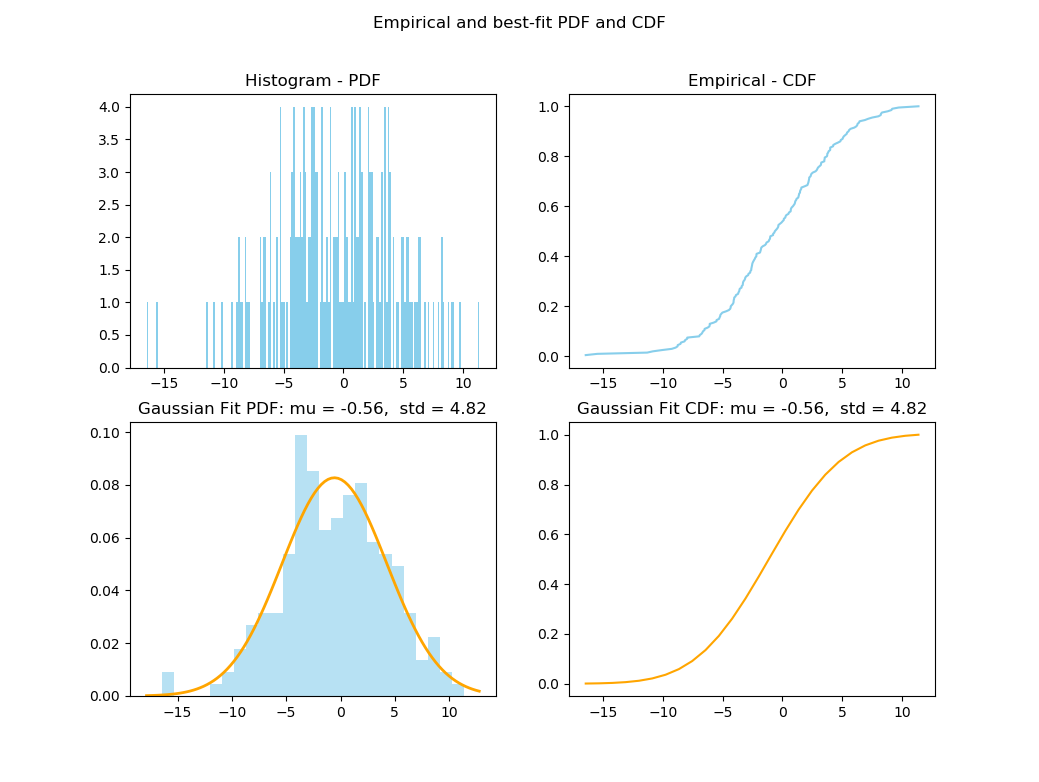
\includegraphics[width=0.8\textwidth]{SectionLetsMath/elemStat_figures/fig_empiricalPdfCdf.png}
\captionsetup{type=figure}
\caption{Empirical and best-fit probability distribution}
\label{fig_empiricalPdfCdf}
\end{figure}

\subsection{Statistical Moments}
As stated before, it is of our interest to infer properties on the random variable to understand the realisations of the related event. Statistical moments are properties that aim at parametrising the shape of a PDF. Let us define the moment of order $m$ as:

\begin{equation}
E\left[\left(x\right)^m\right]=\int_{-\infty}^{+\infty}f\left(x^m\right)dx
\label{eq_momentOfOrderm}
\end{equation}

and the central moment of order m, as:

\begin{equation}
M_m=E[\left(x-\mu\right)^m]
\label{eq_centralMomentOfOrderm}
\end{equation}

The moment of the first order is called \textit{mean} (or expectation) of the probability distribution, generally indicated using the Greek letter $\mu=E[(x)]$.\par

The central moment of the second order is called variance, and it quantifies how much the observations are far from the mean value $\mu$ of the distribution. The variance is represented by $\sigma^2$.We can express the value of $\sigma^2$  by using equation
\ref{eq_momentOfOrderm}.
\begin{equation}
    \label{eq_deploymentVariance}
    \begin{split}
    \sigma^2 & =\ E\left[\left(x-\mu_x\right)^2\right]\\
    & =\int_{-\infty}^{+\infty}\left(t-\mu\right)^2f_xdt=E\left[x^2+\mu^2-2x\mu\right]\\
    & =E\left(x^2\right)+\mu^2-2\mu^2\\
    & =E\left(X^2\right)-\mu^2
    \end{split}
\end{equation}
Usually, we take care of $\sigma=\sqrt{\sigma^2}$ since it has the same unit of measure of $\mu$.\par

Other important central moments (order 3 and 4) are used to describe the shape of a PDF:
\begin{itemize}
    \item $\frac{M_3}{\sigma^3}\ $ is called \textit{skewness};
    \item $\frac{M_4}{\sigma^4}\ $  is called \textit{kurtosis} or \textit{flatness}.
    
\end{itemize}

% INSERT fig_skewnessKurtosis
\begin{figure}[hbt!]
\centering
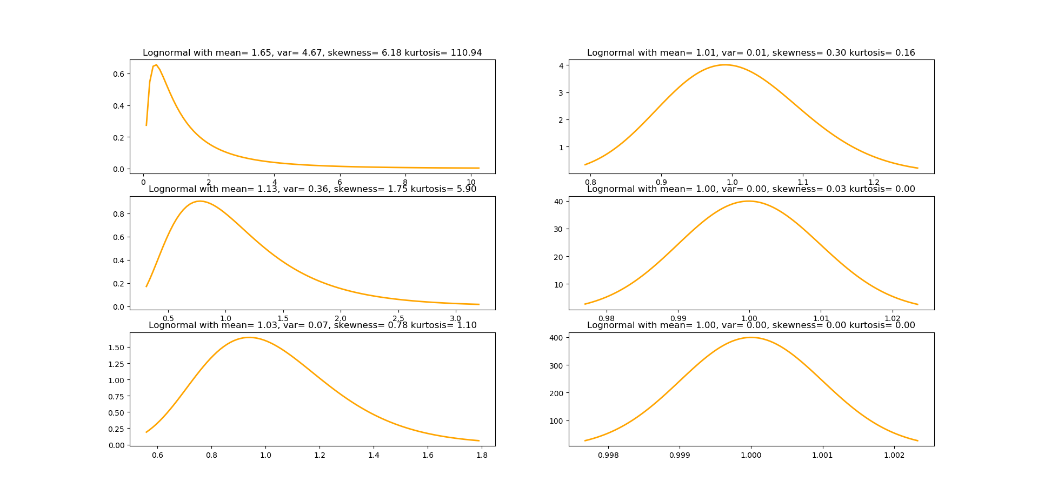
\includegraphics[width=1\textwidth]{SectionLetsMath/elemStat_figures/fig_skewnessKurtosis.png}
\captionsetup{type=figure}
\caption{Skewness and kurtosis of a lognormal distribution.}
\label{fig_skewnessKurtosis}
\end{figure}

Figure \ref{fig_skewnessKurtosis} presents an example of skewness and kurtosis of different distributions (here we use the lognormal). Skewness describes how the mode $M$ of the distribution is far from the mean $\mu$ (positive skewness when $M<\mu$ and negative skewness when $M>\mu$). Kurtosis defines the tailedness of the distribution, higher the kurtosis, higher the relevance of the tails of the distribution.\footnote{The source code of Figure \ref{fig_skewnessKurtosis} is available \href{https://github.com/aletuf93/logproj/blob/master/examples/01_elemStat/01.\%20Probability\%20Theory.ipynb}{here}.
}

\subsection{Covariance and Correlation} \label{secCovarianceCorrelation}
Often, it is necessary to compare the behaviour of two random variables to understand if their related events are somehow correlated. The covariance function $cov(X,Y)$ measures how much two random variables vary together.

\begin{equation}
cov\left(X,Y\right)=E\left[\left(X-E\left[Y\right]\right)\left(Y-E\left[Y\right]\right)\right]=E\left[XY\right]-E[X]E[Y]
\label{eq_covariance}
\end{equation}

The correlation between two random variables is a scalar number defining a measure of their statistical association. The correlation between two random variables is measured normalising the covariance to $\rho_{X,Y}$.

\begin{equation}
\rho_{X,Y}=\frac{cov(X,Y)}{\sigma_X\sigma_Y}
\label{eq_correlation}
\end{equation}

Measuring the correlation between variables is extremely important to evaluate their information content. If two variables are completely correlated (or uncorrelated), their information content is entirely defined by a single of them. Scatterplots are used to visualise correlations. Figure \ref{fig_irisCorrelation} presents an example from the famous \textit{iris dataset}. This dataset is largely used in machine learning examples, and it contains 50 samples for each of the three species of the iris flower (\textit{iris setosa}, \textit{iris virginica} and \textit{iris versicolor}). For each sample, the dataset maps the sepal and petal length and width. A high positive correlation can be easily identified between the variables \textit{petal\_len} and \textit{petal\_wid}.

% INSERT fig_irisCorrelation
\begin{figure}[hbt!]
\centering
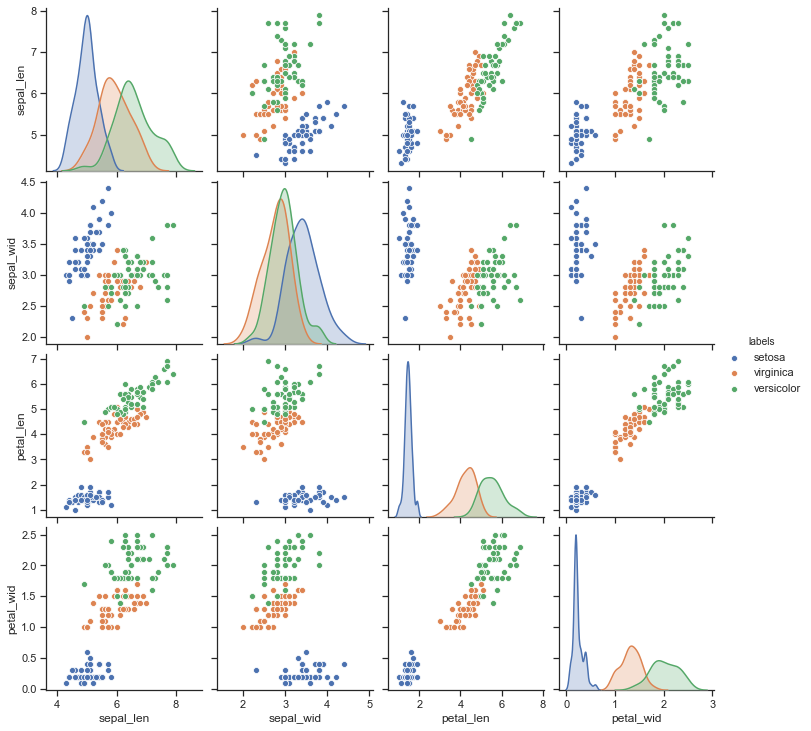
\includegraphics[width=1\textwidth]{SectionLetsMath/elemStat_figures/fig_irisCorrelation.png}
\captionsetup{type=figure}
\caption{Scatterplot of the iris sample dataset.}
\label{fig_irisCorrelation}
\end{figure}

Sometimes, it may be interesting to evaluate how much a single random variable varies with itself. This is the case of a time series that may have some seasonal components. The autocovariance is introduced to meet this goal. It measures how much a random variable varies with itself after some lag $k$ (e.g. a time lag in a time series).

\begin{equation}
\gamma_k=cov\left(X_t,X_{t-k}\right)=E\left[\left(X_t-\mu_t\right)\left(X_{t-k}-\mu_{t-k}\right)\right]-\mu_t\mu_{t-k}
\label{eq_autocovariance}
\end{equation}

Similarly to the variance, it is possible to define a global autocorrelation function (ACF) $\rho_k$ measuring the correlation of a variable $X$ with itself after a time lag $k$. This function expresses the linear dependence between the random variable observed at time $t$ and itself observed at time $t-k$.

\begin{equation}
\rho_k=corr\left(X_t,X_{t-k}\right)=\frac{E[(X_t-\mu_t)(X_{t-k}-\mu_{t-k})]}{\sqrt{Var(X_t)Var(X_{t-k})}}
\label{eq_ACF}
\end{equation}

A partial autocorrelation function (PACF) $\phi_{kk}$ is introduced to measure the linear dependence between the random variable observed at time t and itself observed at time $t-k\ $ without taking into account the intermediate correlations (i.e. $\phi_{kk}$ does not consider the dependence between $X_t$ and $X_{t-1}$ ; $X_t$ and $X_{t-2}$ ; ... ; $X_t$ and $X_{t-k+1}$).

\begin{equation}
\phi_{kk}=Corr(X_t,X_{t-k}|X_{t-1},X_{t-2},\ldots,X_{t-k+1})
\label{eq_PACF}
\end{equation}

Figure \ref{fig_ACFPACF} illustrates a seasonal time series with its ACF and PACF. ACF and PACF of the series evidence that autocorrelation of the realisations exists after about five time lags. Additional details on the use of this information for time series analysis are introduced in Section \ref{secTimeSeries}.\footnote{The source code of Figure \ref{fig_ACFPACF} is available \href{https://github.com/aletuf93/logproj/blob/master/examples/02.\%20Time\%20Series.ipynb}{here}.}

% INSERT fig_ACFPACF
\begin{figure}[hbt!]
\centering
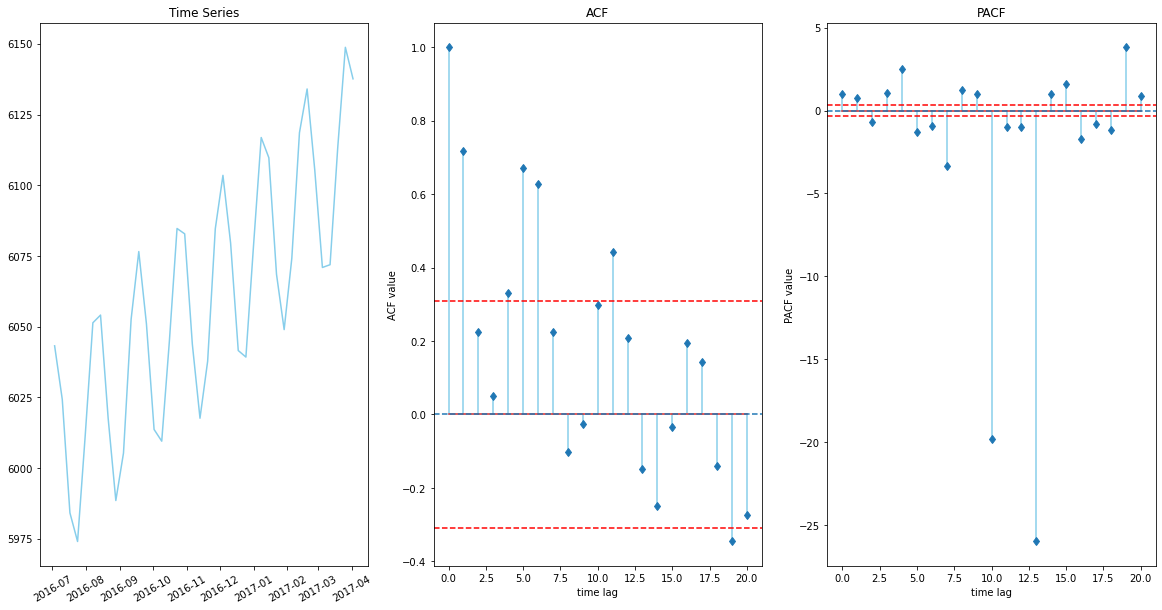
\includegraphics[width=1\textwidth]{SectionLetsMath/elemStat_figures/fig_ACFPACF.png}
\captionsetup{type=figure}
\caption{An example of the ACF and PACF of a time series.}
\label{fig_ACFPACF}
\end{figure}

\subsection{Distance between random variables}
In many applications, it is interesting to have a measure of the distance between two random variables as, for example, the distance between two points on a line, chosen with a law of probability. \par

The distance function is a random variable $Z$ estimated as $Z=|x-y|$. We need to estimate its PDF or CDF to get knowledge about $Z$. By the definition of $F$ we have:

\begin{equation}
F_z\left(z\right)=Prob{\left\{Z\le z\right\}}=Prob\left\{\left|x-y\right|\le z\right\}
\label{eq_Distance1}
\end{equation}

It is necessary to integrate the density function $f_Z$ in the domains $D_X$, and $D_Y$, to calculate $F_Z$.In order to define the domains $D_X$ and $D_Y$, it is necessary to consider the function $Z=\left|X-Y\right|$ on the plan x,y (see Figure \ref{fig_DistanceDomain}).

% INSERT fig_DistanceDomain
\begin{figure}[hbt!]
\centering
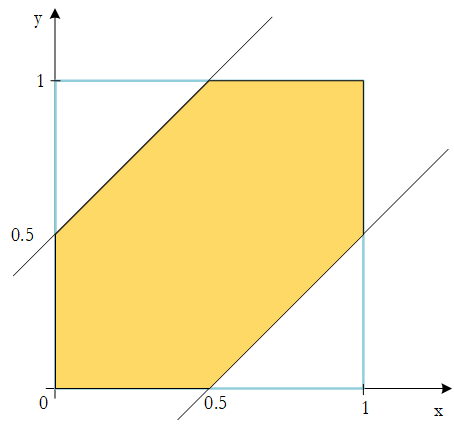
\includegraphics[width=0.7\textwidth]{SectionLetsMath/elemStat_figures/fig_DistanceDomain.png}
\captionsetup{type=figure}
\caption{Domain of the random variable $Z=|X-Y|$}
\label{fig_DistanceDomain}
\end{figure}

The value of $F_Z$ can be determined from the PDF $f_{XY}$.

\begin{equation}
F_z\left(z\right)=\int_{D_X}\int_{D_Y}{f_{xy}\left(x,y\right)dxdy}
\label{eq_Distance2}
\end{equation}

Let assume $X$ and $Y$ being independent\footnote{With the independence hypothesis, $f_{XY}=f_X\bullet f_Y$} and uniformly distributed on $[0,p]$. 

\begin{equation}
    \label{eq_Distance3}
    \begin{split}
    X~U\left[0,p\right];f_x=\frac{1}{p};F_x=\frac{x}{p} \\
    Y~U\left[0,p\right];f_x=\frac{1}{p};F_x=\frac{y}{p} \\
    \end{split}
\end{equation}

The value of $F_Z$ is consequently defined as:

\begin{equation}
F_Z(z)=\int_{D_X}\int_{D_Y}{f_x\left(x\right)f_y(y)dxdy}
\label{eq_Distance4}
\end{equation}

The domain of the function is one out of the three regions of plan defined by the corresponding equalities $Y=X+Z$ , $Y=X-Z$. In Figure \ref{fig_DistanceDomain}, $Z=0.5$. The region is the one between the two lines. It is, then possible to obtain $F_Z$. 
\begin{center}
\begin{equation}
    \label{eq_Distance5}
    \begin{split}
    F_z\left(z\right) =\int_{x=0}^{x=p-z}{\int_{y=0}^{y=z+x}{\frac{1}{p}\times\frac{1}{p}dy\ dx\ }}  + \int_{x=p-z}^{x=z}\int_{y=0}^{y=p}{\frac{1}{p}\times\frac{1}{p}dy\ dx\ }+ \\
    +\ \int_{x=z}^{x=p}{\int_{y=x-z}^{y=p}{\frac{1}{p}\times\frac{1}{p}dy\ dx\ }=} \\
    =\frac{1}{p^2}\left\{\int_{x=0}^{x=p-y}\left(x+z\right)dx+\ \int_{x=p-z}^{x=z}pdx+\ \int_{x=z}^{x=p}\left(p-x+z\right)dx\right\} \\
    =\frac{z\left(2p-z\right)}{p^2} \\
    \end{split}
\end{equation}
\end{center}


The PDF $f_Z$ is defined from equation \ref{eq_cdfIntegralPdf} as follows.

\begin{equation}
f_Z(z)=\frac{dF(z)}{dz}=\frac{2\left(p-z\right)}{p^2}
\label{eq_Distance6}
\end{equation}

We can test that $f_z$ is a PDF since by the definition of $X$,$Y$ its domain is $[0,p]$ and its integral equals 1.

\begin{equation}
f_{Z\left(z\right)}=\int_{0}^{p}\frac{2\left(p-z\right)}{p^2}dz=\left[\frac{2z^2}{2p^2}\right]_0^p=1\ \ 
\label{eq_Distance7}
\end{equation}

At this stage, all the properties of $Z$ are defined by $f$ and $F$. For example, it is possible to calculate the mean value corresponding to the average distance between $X$ and $Y$. 

\begin{equation}
    \label{eq_Distance8}
    \begin{split}
    E\left[Z\right] & =\int_{0}^{p}\frac{2\left(p-z\right)}{p^2}zdz=\frac{1}{p^2}\int_{0}^{p}\left(2pz-{2z}^2\right)dz= \\
    & =\frac{1}{p^2}\left[\frac{2pz^2}{2}-\frac{{2z}^3}{3}\right]_0^p=\frac{1}{p^2}\left[p^3-\frac{2p^3}{3}\right]= \\
    & = \frac{p}{3} \\
    \end{split}
\end{equation}
The procedure above can be applied to any probability distribution of $X$ and $Y$ under the independence hypothesis.

\section{Statistics} \label{secStatistics}

The statistic is an application of the probability theory to infer the properties of a population of elements working on a small subset of it (i.e. a sample). The statistic was born to solve the trade-off between the time necessary to collect data on-field and the accuracy of the information obtained by these data. In fact, it is always impossible to collect all the information available since the population counts thousand or millions of different elements. Statistics provides models to get robust results even when we have few observations of a physical phenomenon.

\subsection{Estimators} \label{secEstimators}

Statistics usually follows a precise workflow:
\begin{enumerate}
    \item Collect data; 
    \item Sample data;
    \item Infer properties from samples to the whole population.
\end{enumerate}

The last step is the one we are interested in the most: we need to estimate the parameters of the probability distribution of the population. Estimators are used to calculating the value of a parameter of a population (e.g., the mean or the variance) based on the observed values given by the sample. Estimators are classified as biased or unbiased. We call an estimator $\hat{\theta}$ of a parameter $\theta$ unbiased when $E\left[\hat{\theta}\right]=\theta$.\par

The most common estimators are needed for the estimation of $\mu\ $ and $\sigma $ of the population. The sample mean $\bar{X}$ is an unbiased estimator of $\mu$ (see equation \ref{eq_sampleMean}). While the sample variance $S^2$ is an unbiased estimator for $\sigma^2$ (see equation \ref{eq_sampleVariance}).

\begin{equation}
\bar{X}=\frac{X_1+\ldots+X_N}{N}
\label{eq_sampleMean}
\end{equation}

\begin{equation}
S^2=\frac{1}{N-1}{\sum_{i}^{N}\left(X_i-\bar{X}\right)^2}
\label{eq_sampleVariance}
\end{equation}

Estimators are evaluated according to their accuracy (i.e. their closeness to the random variable they estimate). In general, we can find two sources of inaccuracy on an estimator: the bias and the variance. Let assume having a model f producing an estimator $\hat{\theta}$ for the random variable $\theta$ with an error $\epsilon$. 

\begin{equation}
\theta \simeq \hat{\theta}=f\left(X\right)+\epsilon
\label{eq_bias1}
\end{equation}
A vector $x_0$ defines a set of realisations of $X$ and we want to define the error of the estimator $\hat{\theta}$.

\begin{equation}
    \label{eq_bias2}
    \begin{split}
    \epsilon\left(x_0\right) = E\left[\left(\hat{\theta}-\hat{f}\left(X\right)\right)^2|X=x_0\right]= \\
     =\ E\left[\left(\hat{\theta}-E\left[\hat{f}\left(x_0\right)\right]+E\left[\hat{f}\left(x_0\right)\right]-\hat{f}\left(x_o\right)\right)^2\right]=\\
     = E[\left(\hat{\theta}-E\left[\hat{f}\left(x_0\right)\right]\right)^2 + \left(E\left[\hat{f}\left(x_0\right)\right]-\hat{f}\left(x_o\right)\right)^2 + \\ 2\left(\hat{\theta}-E\left[\hat{f}\left(x_0\right)\right]\right)\times \left(E\left[\hat{f}\left(x_0\right)-\hat{f}(x_0)\right]\right)]=\\
     =E\left[\left(\hat{\theta}-E\left[\hat{f}\left(x_0\right)\right]\right)^2\right] +E\left[\left(E\left[\hat{f}\left(x_0\right)\right]-\hat{f}\left(x_o\right)\right)^2\right] + \\
     + E\left[2\left(\hat{\theta}-E\left[\hat{f}\left(x_0\right)\right]\right)\left(E\left[\hat{f}\left(x_0\right)-\hat{f}\left(x_0\right)\right]\right)\right]=\\
     Var\left(\hat{f}\left(x_0\right)\right)+\left(E\left[\hat{f}\left(x_0\right)\right]-\hat{f}\left(x_o\right)\right)^2\\
     =Var\left(\hat{f}\left(x_0\right)\right)+\ Bias^2\left(\hat{f}\left(x_0\right)\right)\\
    \end{split}
\end{equation}


The error of an estimator can be defined according to \ref{eq_bias2} using:
\begin{itemize}
    \item 	$Bias^2\left(\hat{f}\left(x_0\right)\right)$ is the squared bias in the estimation of the mean. It describes how much the mean of the estimator is far from the true mean.
    \item 	$Var\left(\hat{f}\left(x_0\right)\right)$ is the deviation of the estimator around its mean.
\end{itemize}

The role of the variance and bias can be easily visually interpreted in Figure \ref{fig_biasVariance}.

% INSERT fig_biasVariance
\begin{figure}[hbt!]
\centering
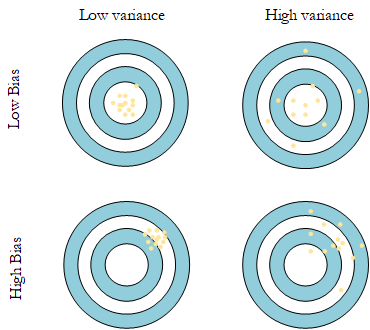
\includegraphics[width=0.7\textwidth]{SectionLetsMath/elemStat_figures/fig_biasVariance.png}
\captionsetup{type=figure}
\caption{The bias and variance of an estimator}
\label{fig_biasVariance}
\end{figure}

Complex prediction models developed using data-driven methods, have to take into account the variance and the bias of the predictions they produce. In particular, there is a bias-variance trade-off. Typically, the more complex the model, the lowest the variance and the highest the bias produced by predictions of the models. On the opposite, a simple model leads to low bias but high variance. Practically speaking, it is always necessary to take into account the bias and the variance of the response of a model to check if it fits with its purpose. Developing a complex model to solve a simple problem is just a way to add additional variance to the responses of the model. In general, we keep a model as simpler as possible (according to the Ockham's razor principle). \par

We introduce the Gauss-Markov theorem to show an important property of the linear regression estimator (see chapter \ref{chapLinearRegression}). Let $\hat{\theta}=c^Ty$ be an unbiased estimator of:

\begin{equation}
\alpha^T\beta=\alpha^T\left(X^TX\right)^{-1}X^Ty
\label{eq_biasLinearRegression1}
\end{equation}

Then:

\begin{equation}
E\left[c^Ty\ \right]=\alpha^T\beta
\label{eq_biasLinearRegression2}
\end{equation}

\begin{equation}
Var\left(\alpha^T\hat{\beta}\right)\le Var(c^Ty\ )
\label{eq_biasLinearRegression3}
\end{equation}

The \ref{eq_biasLinearRegression1} is the expression of a linear regression of $\theta=\alpha^T\beta$. In other words, a linear regression  provides the lowest variance estimator possible. The lowest variance does not imply a lower error in the prediction since we have no information about the other error component (i.e. the bias). Nevertheless, we should prefer linear regression, that is a very simple model, when we are sure there is no bias, i.e. $E\left[E\left[\hat{\theta}\right]-\theta\right]^2=0$. In other words, when the world behaves linearly, use a linear model.

\subsection{Maximum Likelihood Inference}
In many practical cases, we need to get a good estimate of a parameter $\theta$ of a PDF, given a sample of the population. Maximum likelihood estimation (MLE) is the tool to do that. We define a function $g_\theta(z)$; where $g$ is the PDF (e.g., normal distribution) of $z_i$ and $\theta$ are the unknown parameters to estimate (e.g. the mean and the variance $\mu$, $\sigma^2$). We need to find values of $\theta$ such that they properly represent the statistical sample. This equals to imply the maximisation of a likelihood function $L$.

\begin{equation}
L\left(\theta,\ Z\right)=\prod_{i=1}^{N}{g_\theta(z_i)}
\label{eq_MLE1}
\end{equation}

The maximisation is done by considering the logarithm of $L$. Maximising $L$ will maximise $\log(L)$ too, due to the monotony of the logarithm. To get a maximum likelihood estimation, we need to maximise:

\begin{equation}
l\left(\theta,Z\right)=\sum_{i=1}^{N}{l\left(\theta,z_i\right)=\sum_{i=1}^{N}\log{\left(g_\theta\left(z_i\right)\right)}}
\label{eq_MLE2}
\end{equation}

This is done by looking for $\theta$ maximising the function:

\begin{equation}
\dot{l}\left(\theta,Z\right)=\ \sum_{i=1}^{N}{\dot{l}\left(\theta,z_i\right)=\sum_{i=1}^{N}{\frac{\partial l\left(\theta,z_i\right)}{\partial\theta}=0}}
\label{eq_MLE3}
\end{equation}
In practical cases, it may be difficult to express the formula of the PDF $g$ and to calculate its derivative to get an MLE. Computerised algorithms have been implemented to solve this problem by approximation where it is not possible to solve it analytically. Bootstrap and Montecarlo simulation are common examples.

\subsection{Kernel Density Estimation} \label{secKernelDensityEstimation}
The estimation of a PDF, can be obtained using a graphic methodology, instead of mathematically define its parameters. Having a set of empirical observations, it is always possible to use a histogram to represent its frequency analysis. The width of each bin of the histogram defines the shape of the curve. Figure \ref{fig_empiricalBinning} shows different histograms of the same empirical sample by using different widths of the histogram bins.\footnote{The source code of Figure \ref{fig_empiricalBinning} is available \href{https://github.com/aletuf93/logproj/blob/master/examples/03.\%20Statistics.ipynb}{here}.
}

% INSERT fig_empiricalBinning
\begin{figure}[hbt!]
\centering
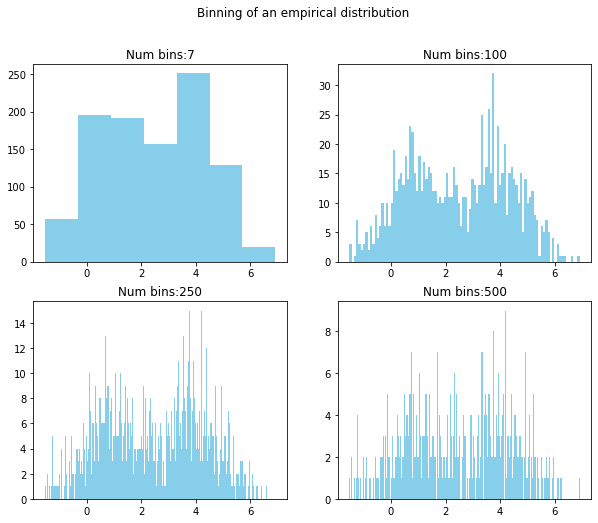
\includegraphics[width=0.7\textwidth]{SectionLetsMath/elemStat_figures/fig_empiricalBinning.png}
\captionsetup{type=figure}
\caption{Definition of histograms with different bin size}
\label{fig_empiricalBinning}
\end{figure}

Kernel Density Estimation (KDE) is a procedure to estimate the PDF of a random variable based on its observations. The idea is to define the shape of the PDF based on the empirical values smoothed around a local region $b$ called bandwidth. This is similar to the choice of the number of bins to define a histogram. KDE can be expressed as:

\begin{equation}
\hat{f}=\frac{1}{n}\sum_{i}^{n}K\left(\frac{x-x(i)}{b}\right)
\label{eq_KDE}
\end{equation}

Where K is a kernel function with a peak on 0 (it is common to use a gaussian function). Figure \ref{fig_KDE} shows the effect of different KDEs with several values of b. \footnote{The source code of Figure \ref{fig_KDE} is available \href{https://github.com/aletuf93/logproj/blob/master/examples/03.\%20Statistics.ipynb}{here}.}

% INSERT fig_KDE
\begin{figure}[hbt!]
\centering
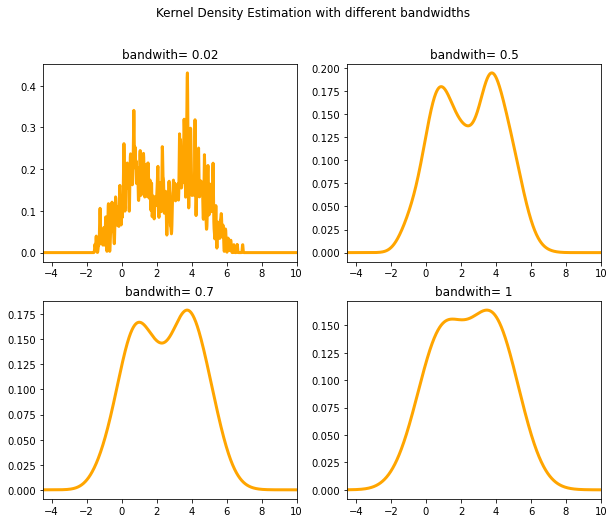
\includegraphics[width=0.7\textwidth]{SectionLetsMath/elemStat_figures/fig_KDE.png}
\captionsetup{type=figure}
\caption{KDE with different bandwidths to estimate the PDF of an empirical sample.}
\label{fig_KDE}
\end{figure}

\subsection{Bootstrapping method} \label{secBootstrapping}

Bootstrapping is an algorithm used to estimate the value of a parameter $\alpha$ (e.g. the mean or variance) from a population where its PDF is unknown or too difficult to estimate analytically.  Let X be a set of observations with cardinality $n$. Algorithm \ref{algo_bootstrap} illustrates the Bootstrapping method.

\begin{algorithm}[H]
\DontPrintSemicolon
\SetAlgoLined
Set the number of iterations B\;
\For{$i=1:B$}{
    Set $\beta$ = $n$ points randomly picked from $X$. \;
    Use $\beta$ to estimate the parameter $\alpha$. \;
}
Define the confidence interval of $\alpha$ using the statistic of the $B$ iterations; $\bar{\alpha}=\frac{1}{B}\sum_{i=1}^{B}\alpha_i$ \;
\caption{Bootstrapping algorithm}
\label{algo_bootstrap}
\end{algorithm}

\subsection{Montecarlo method} \label{secMontecarlo}
Montecarlo simulation is a valid alternative to measure the outcome of a process where many random variables with given PDF are involved, but their joint distribution is hard to compute. \par

Let consider the random variables $X_i$ $i=1,\ldots,q$ whose distribution are given and $\alpha=f(X_i)$. We need to infer properties on the distribution of $\alpha$. Algorithm \ref{algo_montecarlo} shows the Montecarlo simulation to estimate the distribution of $\alpha$. 

\begin{algorithm}[H]
\DontPrintSemicolon
\SetAlgoLined
Set the number of iterations M\;
\For{$i=1:M$}{
    Sample the value for each $X_i$, $i\in q$ according to their PDFs \;
    Evaluate $\alpha=f(X_i)$  \;
}
Define the confidence interval of $\alpha$ using the statistic of the $M$ iterations; $\bar{\alpha}=\frac{1}{M}\sum_{i=1}^{M}\alpha_i$ \;
\caption{Montecarlo algorithm}
\label{algo_montecarlo}
\end{algorithm}

\subsection{Data collection and Measurement systems} \label{secMeasurementSystem}
Dealing with empirical data, it is always necessary to define a measurement system to pick accurate data on-field. If the measurement system is not accurate or not precise, all the following analyses will keep an underlying error. A measurement system determines the measured value $X_1$ of a realisation $X_{true}$. Having:

\begin{equation}
X_1=X_{true}+\beta+\epsilon
\label{eq_measurement1}
\end{equation}

Where $X_{true}$ is the real value of the variable; $\beta$ is the bias (accuracy or systematic error), i.e. how much far the (average value) of the measure from $X_{true}$; $\epsilon$ are random errors depending on the precision of the measurement system. A good measurement procedure has:

\begin{equation}
\mu=\lim_{N \to +\infty}{\frac{1}{N}\sum_{i=1}^{N}{X_i=X_{true}+\beta}}
\label{eq_measurement2}
\end{equation}

\begin{equation}
\lim_{N \to +\infty}{\frac{1}{N}\sum_{i=1}^{N}{\epsilon_i=0}}
\label{eq_measurement3}
\end{equation}

The analysis of uncertainty aims at the definition of $\beta$ and $\epsilon$ of data collected on-field, providing methods to handle and process empirical data correctly.

\subsubsection{Systematic errors}
Systematic error (or bias errors) is determined by a measure of the accuracy of the measurement instrument. Systematic errors occur when an instrument has not an appropriate level of accuracy compared to the variable one wants to measure. For example, it is inadequate to measure the length of a warehouse rack using a ruler. A measurement instrument always requires calibration to be accurate. For example, using a calliper, the systematic error is often linked to a wrong calibration. 

\subsubsection{Uncertainty errors}
Uncertainty error (or random errors) is a measure of precision linked with the random nature of the measurement process. This is unavoidable and must be normally distributed in any empirical data collection (e.g., the processing time of a part on a workbench should be normally distributed when the process is under control).

\subsubsection{Mistakes}
Mistakes are data points with wrong values. They may be error storing the results of an experiment or outliers which must be deleted when there are solid arguments against the value of these data points.

\subsubsection{Data cleaning}
The process of cleaning data implies deleting data points whose value is outside the limit of the analysis one wants to perform. In particular, it often happens to have outliers whose measure is due to errors, having no connection with the real measure. We introduce two methodologies to deal with outliers.\par

The Chauvenet’s criterion provides a simple method to deal with outliers assuming that data have a Gaussian distribution with mean $\mu$ and standard deviation $\sigma$. Let consider a point $i$ with value $x_i$ to be suspect of being an outlier. Its $t$-value is defined as $t_i=\frac{|x_i-\mu|}{\sigma}$. Chauvenets’ criterion considers the probability that $i$ is found inside or outside a probability band defined as $P=1-\frac{1}{2N}$; where $N$ is the number of samples. Chauvenet’s criterion defines $z=Prob\left(t_i\sigma\notin P\right)\times N$. If $z<0.5$ the point should be rejected. In other words, if a point $i$ is too far from the mean of the normal distribution associated with the sample, it should be rejected. \footnote{The source code of the Chauvenet's method is available \href{https://github.com/aletuf93/logproj/blob/master/logproj/ml_dataCleaning.py}{here}.
} \par
The second methodology we introduce to deal with outliers is the interquartile range (IQR). The IQR method considers the range between the $25^{th}$ and the $75^{th}$ percentile of the data points to detect outliers. In particular, being $IQR = Q_3 - Q_1$, where $Q_1$, and $Q_3$ are the first and the third quartile (equivalent to the $25^{th}$, and the $75^{th}$ percentiles), outliers are found below $Q_1 - (1.5\times IQR)$, and above $Q_3 + (1.5\times IQR)$.\footnote{The source code of the IQR method is available \href{https://github.com/aletuf93/logproj/blob/master/logproj/ml_dataCleaning.py}{here}.
}


\section{Statistical Distributions}
This section introduces the relevant statistical distribution for the applications in the field of logistics and operations.

\subsection{The Normal distribution}
The most important probability distribution is called normal (or Gaussian) distribution, and its PDF is defined as:

\begin{equation}
f\left(X\right)=\frac{e^{-\frac{(X-{\mu)}^2}{2\sigma^2}}}{\sigma\sqrt{\left(2\pi\right)}}
\label{eq_pdfGaussian}
\end{equation}

Having mean $\mu=\sum_{i=1}^{N}\frac{x_i}{N}$, and standard deviation $\sigma=\left[\frac{1}{N}\sum_{i}^{N}\left(X_i-\mu\right)^2\right]^\frac{1}{2}$. When the distribution has a large standard deviation, its peak tends to be lower.\par
The Normal distribution is characterized by a concentration of the observation around the mean. It is possible to control the density of the function with reference to the distance from the mean $\mu$ expressed in terms of the number of standard deviations $\sigma$ (Figure \ref{fig_normal}).

% INSERT fig_normal
\begin{figure}[hbt!]
\centering
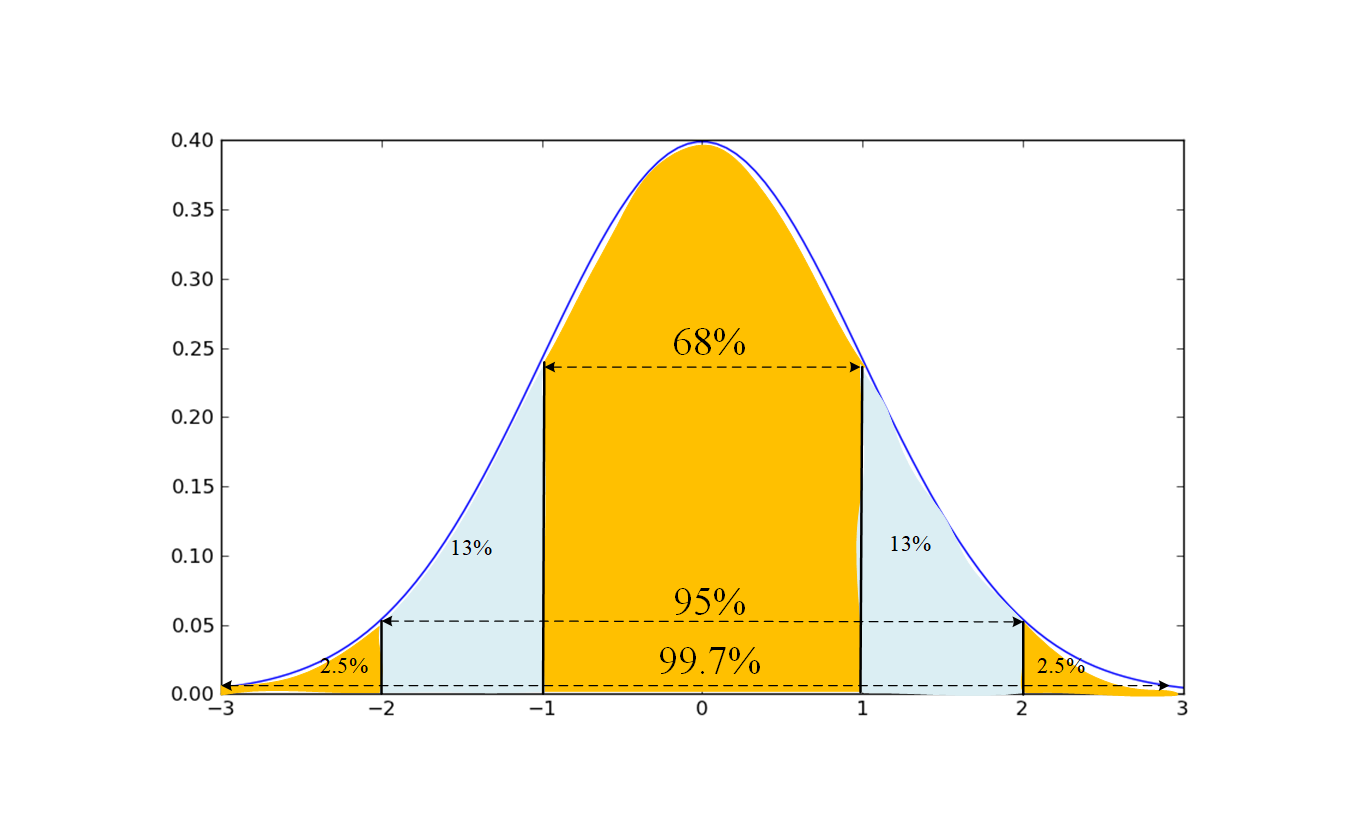
\includegraphics[width=0.9\textwidth]{SectionLetsMath/elemStat_figures/fig_normal.png}
\captionsetup{type=figure}
\caption{Normal distribution probability distribution function (PDF).}
\label{fig_normal}
\end{figure}

When a random variable $X$ is normally distributed, we can prove that there is a  probability equal to $0.95$ that its mean value is found within a confidence interval of $1.96\sigma$.

\begin{equation}
Prob\left\{-1.96\le\frac{X_i-\mu}{\sigma}\le1.96\right\}=0.95
\label{eq_pdfConfidenceInterval1}
\end{equation}

\begin{equation}
Prob\left\{X_i-1.96\sigma\le\mu\le X_i+1.96\sigma\right\}=0.95
\label{eq_pdfConfidenceInterval2}
\end{equation}

A normal distribution has many useful properties. In practice, it is necessary to prove that a sample is normally distributed (e.g. using statistical tests see \ref{secStatTest}) to apply all the magical properties of the normal distribution. This way, by estimating the $\sigma$ of the populations using the estimator $s=\frac{1}{N-1}\sum_{i=1}^{N}{{{(X}_i-\bar{X})}^2\ \ }$, the mean value $\mu$ of the population will have a confidence interval of 95\% within the range $\pm1.96\sigma$. The central limit theorem generalises these properties of the normal distribution to any statistical distribution.

\subsection{Central limit theorem}
The central limit theorem states that describing an event with a sufficiently large number $N$ (with $N\geq30$) of random variables $X_i$, the arithmetic mean of these variables is normally distributed.

\begin{equation}
\bar{x}=\frac{X_1+X_2+\ldots+X_N}{N} \sim N(\mu,\sigma)
\label{eq_centralLimitTheorem}
\end{equation}



In other words, no matter the distribution of the random variables $X_i$, increasing the number of experiments measuring $X_i$, there is a random variable describing the mean value of the experiments, and it is normally distributed.

\subsection{Multivariate normal distribution}
The multivariate normal distribution generalizes the univariate normal distribution to a multidimensional space. Assume $X=\left(X_1,\ldots,X_p\right)^T$ be a $p$-dimensional random vector. $X$ is distributed as a multivariate normal distribution when its density function is as follows.

\begin{equation}
X\sim N_p\left(\mu,\Sigma\right)= f\left(x_1,\ldots,x_p\right)=\frac{1}{\left(2\pi\right)^\frac{p}{2}\left|\Sigma\right|^\frac{1}{2}}e^{-\ \frac{1}{2}\left(x-\mu\right)^T\Sigma^{-1}(x-\mu)}
\label{eq_multivariateNormal}
\end{equation}

Where $\mu$ is the mean vector $\mu=E\left[X\right]=\left[E\left[X_1\right],E\left[X_2\right],\ldots,E\left[X_p\right]\right]^T$ and $\Sigma$ is a $p\times p$ covariance matrix $\Sigma_{i,j}=E\left[\left(X_i-\mu_i\right)\left(X_j-\mu_j\right)\right]=Cov[X_i,X_j]$.

\subsection{The Poisson Distribution} \label{secPoisson}
The Poisson distribution is a discrete probability distribution useful to describe the realisations of events when the average time between the event is given, but the interarrival time between the events is random. This situation is common when dealing with queues (the average throughput of the resource is given, but the interarrival time of the workload is random) or maintenance (the mean time to failure is given, but the exact failure time is unknown). The Poisson distribution has PDF:

\begin{equation}
Prob\left(X=k\right)=\frac{\lambda^ke^{-\lambda}}{k!}
\label{eq_poissonPDF}
\end{equation}

The Poisson distribution identifies the probability of realisation of k events within a time interval $\tau$ having an average number of event per time unit $d$, where $\lambda=d\tau$. Figure \ref{fig_poisson} identifies the shape of the PDF of the Poisson distribution using different values of $\lambda$.\footnote{The source code of Figure \ref{fig_poisson} is available \href{https://github.com/aletuf93/logproj/blob/master/examples/03.\%20Statistics.ipynb}{here}.
}


% INSERT fig_poisson
\begin{figure}[hbt!]
\centering
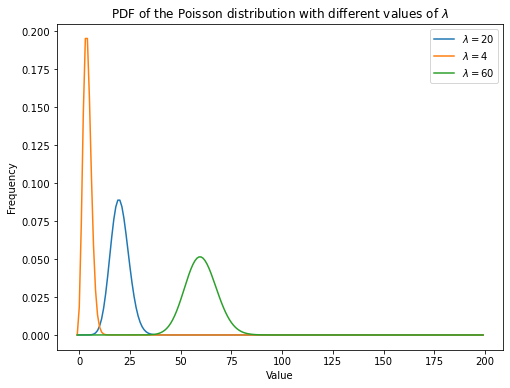
\includegraphics[width=0.9\textwidth]{SectionLetsMath/elemStat_figures/fig_poisson.png}
\captionsetup{type=figure}
\caption{Poisson distribution probability distribution function (PDF).}
\label{fig_poisson}
\end{figure}

\subsection{The Triangular Distribution}
Some times empirical measurements are done on the minimum, maximum and average value of a random variable $X$. In these situations, we have only three values to infer the properties of the random variable $X$. Triangular distribution assumes $X$ having a density with a triangular shape with its mode in correspondence of the mean value, and the vertices at the minimum and maximum values. The triangular distribution has PDF:

\begin{equation}
f(X)=\left\{
                \begin{array}{ll}
                  0\ \ & if\ X<a,\\
                  \frac{2(X-a)}{(b-a)(c-a)}\ & if\ a\le X\le c,\\
                  \frac{2}{b-a}\ & if\ X=c,\\
                  \frac{2(b-X)}{(b-a)(b-c)}\ & if\ c<X\le b,\\
                  0\ & if\ b<X
                \end{array}
              \right.
\label{eq_triangularDF}
\end{equation}

Where $a$ is the minimum value, $b$ is the maximum value, and $c$ is the mean value. Figure \ref{fig_triangular} shows the shape of a triangular distribution.\footnote{The source code of Figure \ref{fig_triangular} is available \href{https://github.com/aletuf93/logproj/blob/master/examples/03.\%20Statistics.ipynb}{here}.
}

% INSERT fig_triangular
\begin{figure}[hbt!]
\centering
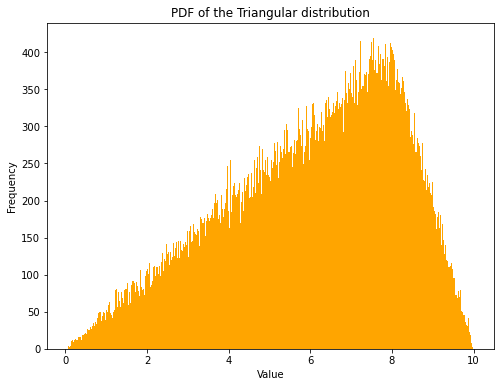
\includegraphics[width=0.9\textwidth]{SectionLetsMath/elemStat_figures/fig_triangular.png}
\captionsetup{type=figure}
\caption{Triangular distribution probability distribution function (PDF).}
\label{fig_triangular}
\end{figure}

\section{Statistical tests} \label{secStatTest}

All the statistical tools introduced so far have been used with a descriptive purpose, i.e. to describe the behaviour of an experiment. At some point, it may be necessary to use statistical tools to get answers about the validity of a theory (e.g. a research intuition). Statistical tests are used for this reason. A statistical test checks if a “test distribution” (e.g., Gaussian, $t$, $\chi^2$) fits with the empirical data. The workflow of a statistical test is as follows.
\begin{enumerate}
    \item Identify the problem and the parameters of interests;
    \item State the null hypothesis $H_0$;
    \item State the alternative hypothesis $H_1$;
    \item Identify a level of significance $\alpha$;
    \item Choose an appropriate statistical test;
    \item Define the rejection region for the null hypothesis;
    \item Compute the test and check whether $H_0$ should be rejected or not.
\end{enumerate}

$H_0$ (or, more often $H_1$) is the hypothesis (e.g. the research intuition one wants to test). Engineeringly speaking, $H_0$ is often formulated as the opposite of what one wants to test. Such that, rejecting $H_0$ is a successful test since it supports the initial thesis.\par

A typical null hypothesis is that there are no differences between two parameters (e.g., the means $\mu_1$ and $\mu_2$) observed from two populations (i.e. they have the same distribution and the differences between them are only due to the chance). The hypothesis is tested within a certain level of significance $\alpha$. Any statistical test works calculating a probability $p$ called $p$-value.\par

The $p$-value is the probability of obtaining an empirical result more extreme than the observed ones due to the sample variability, assuming $H_0$ being true. In other words, the $p$-value is an estimation of the probability that rejecting the null hypothesis is only due to the chance. A high $p$-value may be due to a bad selection of the sample (e.g., too small) while a low $p$-value suggests the significance of the test.\par

For a random variable $X$ with unknown distribution, we observe a value $x$. The calculation of $p$-value is:

\begin{equation}
p=Prob\left\{ X\le x|H_0\right\}
\label{eq_pvalue}
\end{equation}

Figure \ref{fig_StatTest} shows an example where $X$ is an unknown distribution that is tested to have the same mean $\mu$ of the represented normal distribution. The null hypothesis $H_0$ is that \textit{“the empirical data are normally distributed”}. In the figure on the left, the sample with mean value $X$ is too far from the mean of the distribution and the p-value is low; for this reason, $H_0$ is rejected. Otherwise, in the figure on the right, the sample with mean $X$ behaves as the distribution (within the confidence interval of the test $\alpha=0.05$), the $p$-value is higher than $\alpha$, and $H_0$ is not rejected.

% INSERT fig_StatTest
\begin{figure}[hbt!]
\centering
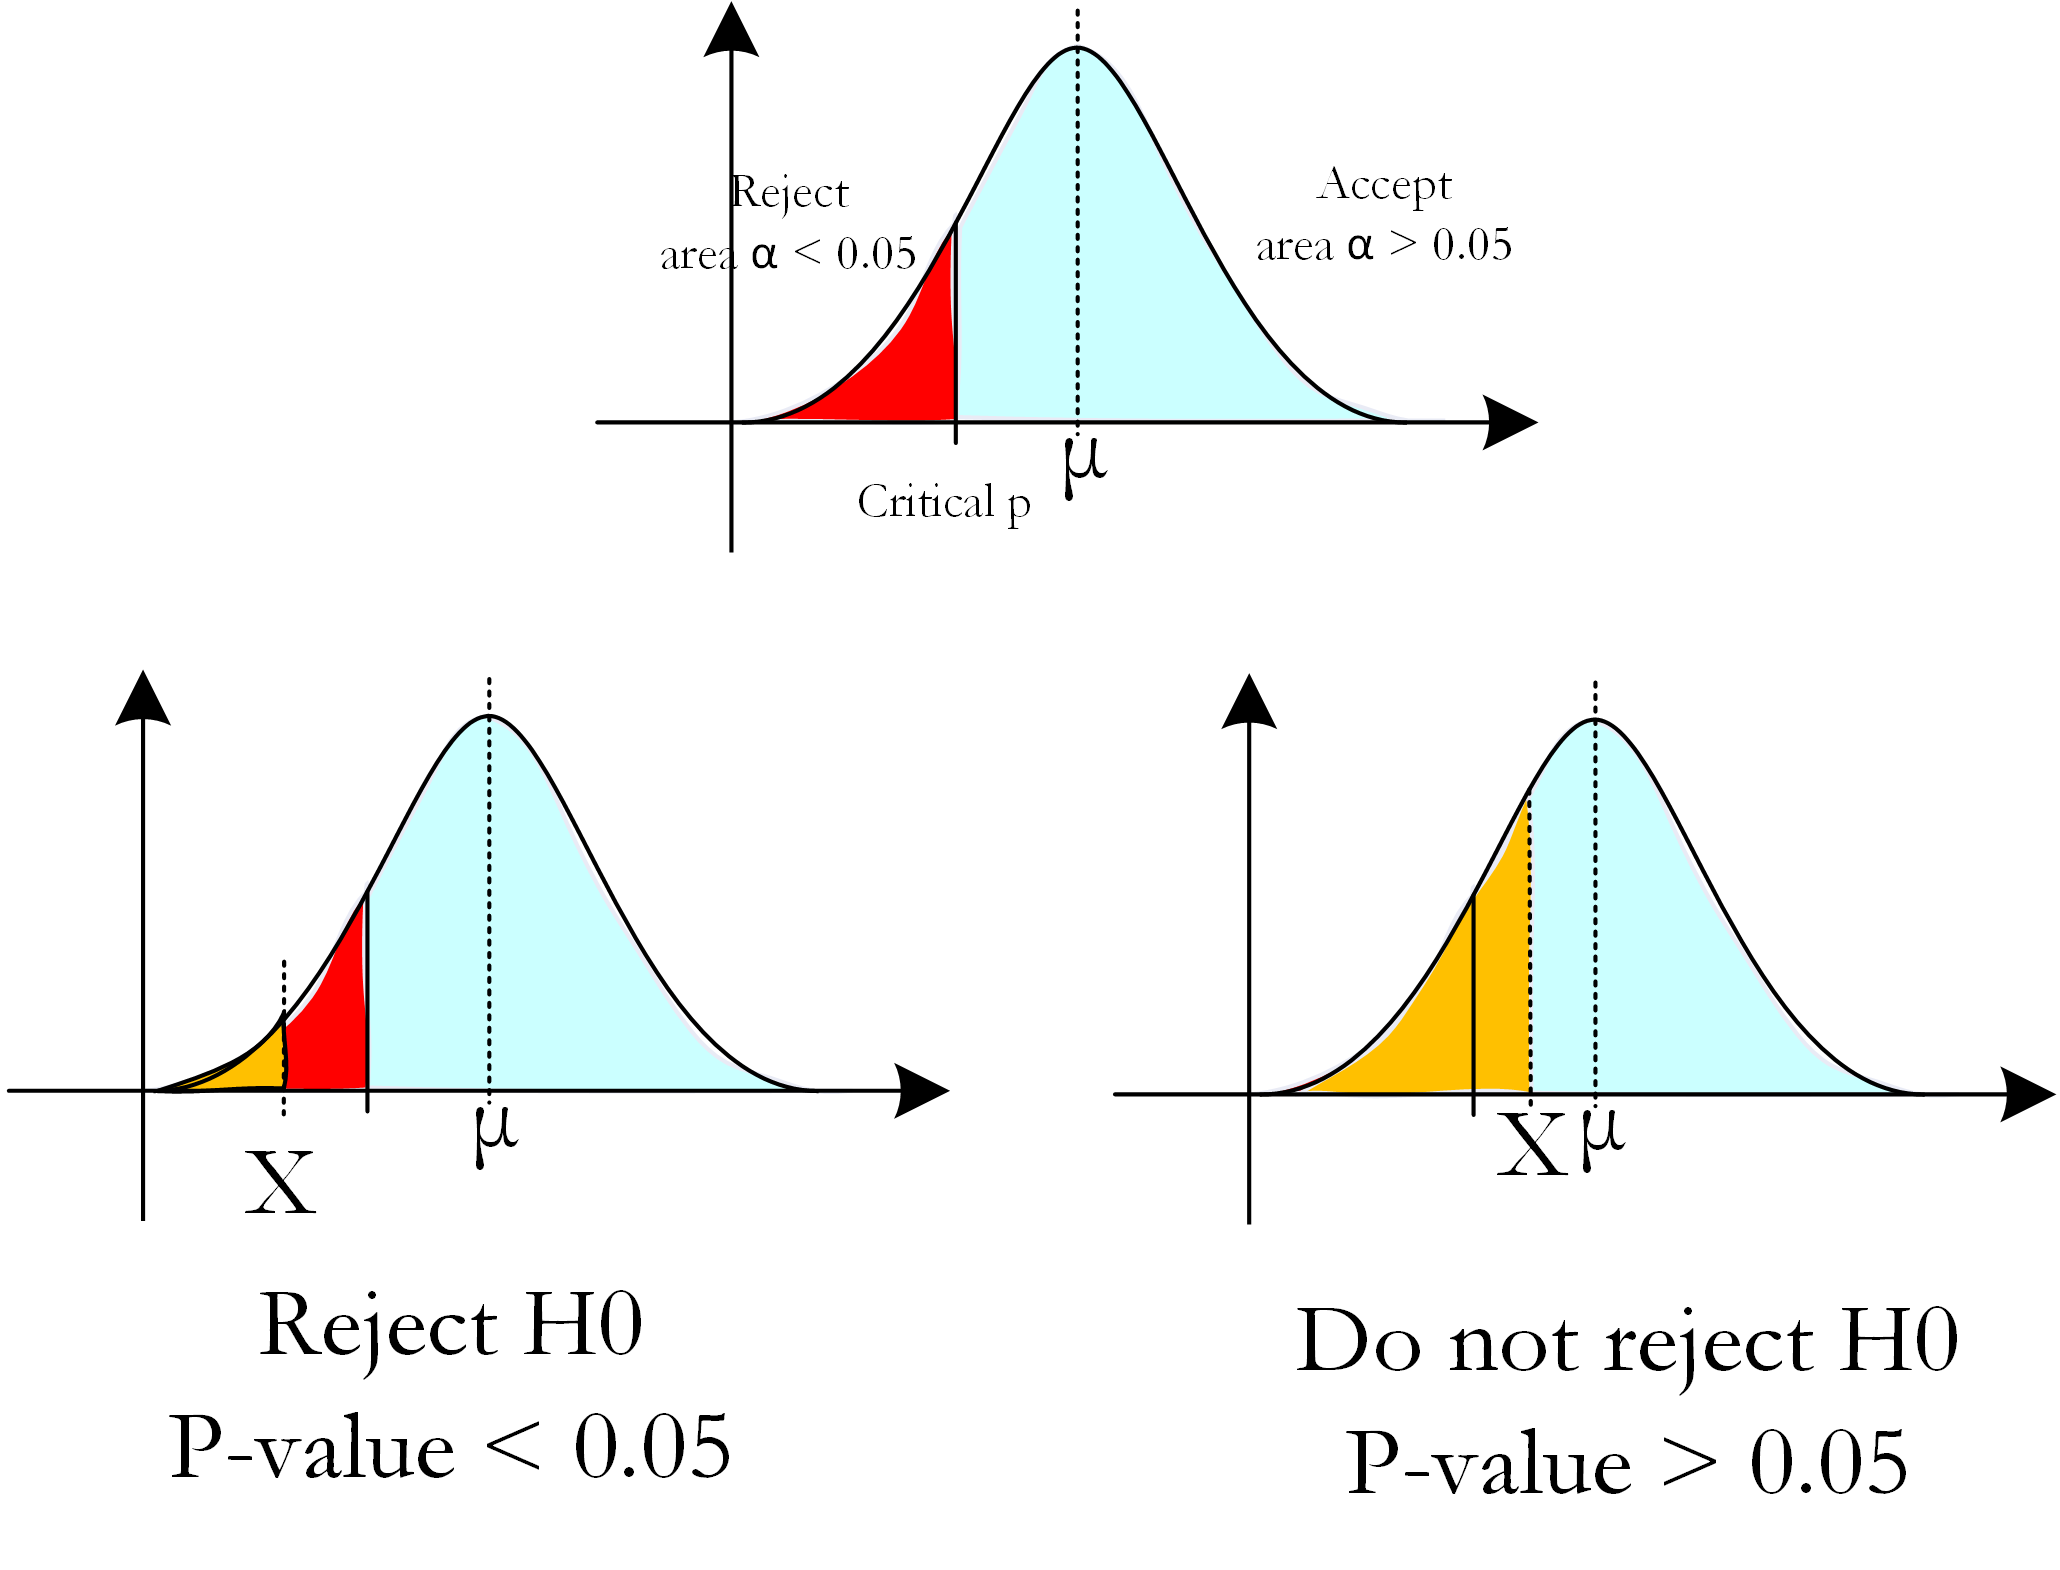
\includegraphics[width=0.9\textwidth]{SectionLetsMath/elemStat_figures/fig_StatTest.png}
\captionsetup{type=figure}
\caption{Graphical representation of a statistical test.}
\label{fig_StatTest}
\end{figure}

The significance of the test depends on the value of $\alpha$ chosen for the test. Table \ref{tab_statTest} shows some common values of $\alpha$ used to accept or discard hypothesis. Please note that $\alpha$ has to be chosen before the test depending on the context and the level of significance expected from the decision-maker. It is a bad practice to make an experiment and afterwards evaluate its results depending on the $p$-value.

% INSERT tab_statTest
\begin{figure}[hbt!]
\centering
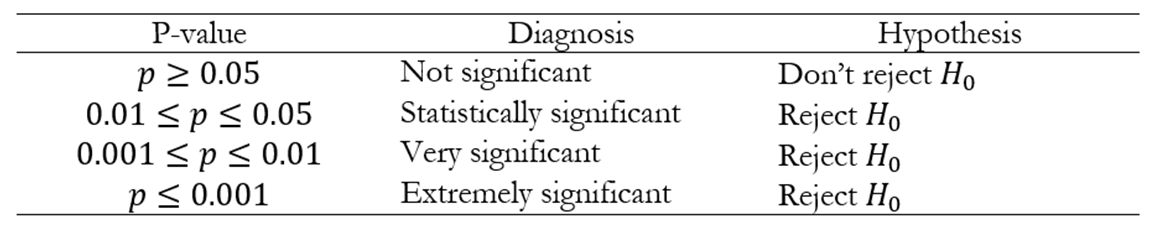
\includegraphics[width=0.9\textwidth]{SectionLetsMath/elemStat_figures/tab_statTest.png}
\captionsetup{type=table}
\caption{$p$-value and levels of significance.}
\label{tab_statTest}
\end{figure}

\subsection{Z-test (normal distribution)}
$Z$-test is used to check if the mean value of a sample is equal to a reference value. In other words, given the value of $\sigma$, one wants to check how far is the sample mean $\bar{X}$ from the population mean $\mu$. Table \ref{tab_zTest} lists the summary of the $Z$-test.


% INSERT tab_zTest
\begin{figure}[hbt!]
\centering
\includegraphics[width=0.9\textwidth]{SectionLetsMath/elemStat_figures/tab_zTest.png}
\captionsetup{type=table}
\caption{Z-test summary.}
\label{tab_zTest}
\end{figure}

$Z$-test assumes a normal distribution and evaluates the $Z$-score of the distribution. The statistic of the test is as follows.

\begin{equation}
Z=\frac{\bar{X}-\mu}{\sigma/\sqrt n}
\label{eq_ztest}
\end{equation}
where $n$ is the number of samples. If $Z<-1.96\ OR\ Z>1.96$ $H_0$ is rejected. The $p$-value is higher than $0.05$ and the value of $\bar{X}$ is too far from $\mu$. If $-1.96\le Z\le1.96$ $H_0$ is accepted since $\bar{X}$ falls within the acceptance region. When the value of $\sigma$ is unknown, or the sample size is too small ($n<30$), a similar test can be performed using a $t$-test.

\subsection{t-test}
The $t$-test aims at checking if a sample behaves like a normal distribution when the sample size $n$ is small. In other words, dealing with a small sample it is important to check if it is possible to apply normal distribution statistics or if the sample belongs to a different distribution. In practice, it is necessary to compare the sample mean $\bar{X}$ and the population mean $\mu$. Since the population variance is unknown, it is assumed $\sigma^2=s^2$ i.e., the variance of the population equals the variance of the sample. The $t$-student distribution measures the difference between the sample mean and the population mean. The statistic of the test follows this distribution.

\begin{equation}
t=\frac{(\bar{X}-\mu)}{s/\sqrt n}
\label{eq_tTest}
\end{equation}

Where $n$ indicates the number of samples i.e., the degree of freedom of the distribution. Consequently , the $t$-distribution has a different shape for different degrees of freedom (see Figure \ref{fig_tDist}).\footnote{The source code of Figure \ref{fig_tDist} is available \href{https://github.com/aletuf93/logproj/blob/master/examples/03.\%20Statistics.ipynb}{here}.} When the number of samples $n$ (i.e. the degrees of freedom) approaches $30$, the $t$-distribution has the same shape of the normal distribution. Table \ref{tab_tTest} illustrates the summary of this test.

% INSERT fig_tDist
\begin{figure}[hbt!]
\centering
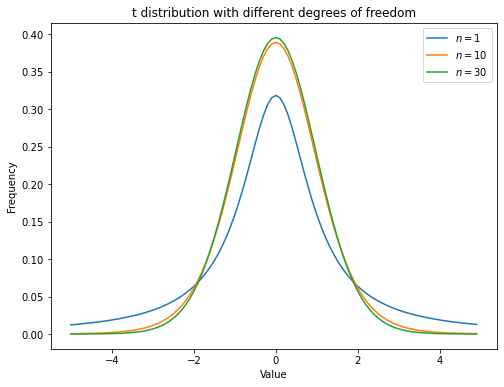
\includegraphics[width=0.9\textwidth]{SectionLetsMath/elemStat_figures/fig_tDist.png}
\captionsetup{type=figure}
\caption{PDF of the $t$-distribution with different degrees of freedom.}
\label{fig_tDist}
\end{figure}

% INSERT tab_tTest
\begin{figure}[hbt!]
\centering
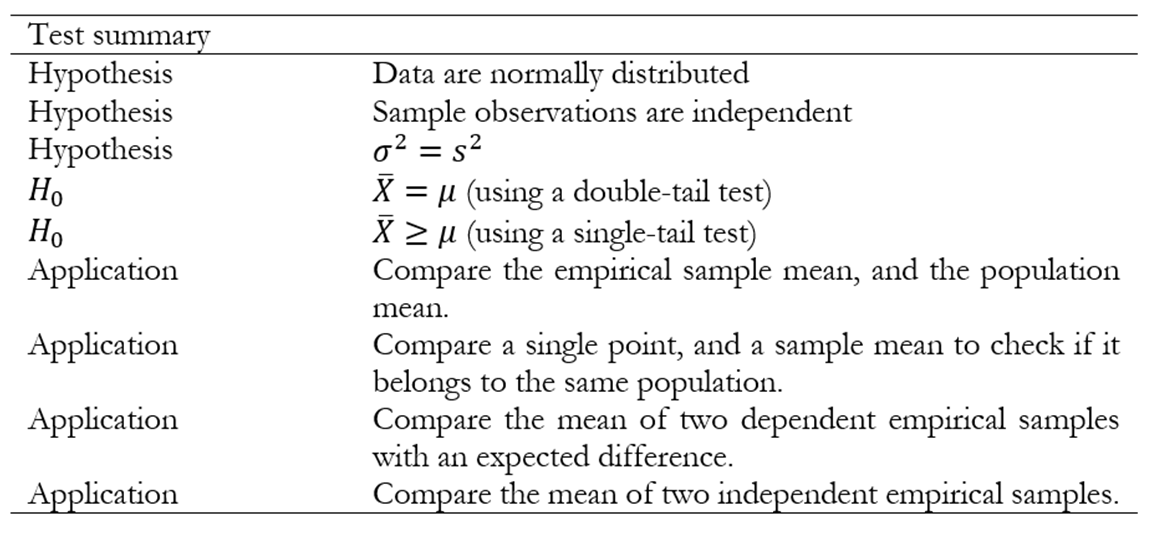
\includegraphics[width=0.7\textwidth]{SectionLetsMath/elemStat_figures/tab_tTest.png}
\captionsetup{type=table}
\caption{$t$-test summary.}
\label{tab_tTest}
\end{figure}

\subsection{$\chi^{2}$-test}
This test is used to check if a sample is distributed according to a given statistical distribution. The distribution of the test is a $\chi^2$ distribution defined as:

\begin{equation}
\chi_k^2=\sum_{i=1}^{k}{x_i^2=x_1^2+\ldots+x_k^2}
\label{eq_chi2Distribution}
\end{equation}

$x_1,\ldots x_k$ are random variables normally distributed and $k$ is the number of degrees of freedom. To check if a sample fits a statistical distribution (e.g., a normal distribution), the events are divided into $k$ subset each one having an observed frequency $o_k$ (sample) and an expected frequency $e_k$ (from the distribution). The definition of the $k$ classes is very important. The more the classes, the more one can check the fit with a statistical distribution. A good rule is that \% of the classes has at least 5 items and no class is empty. The statistic of the test is calculated as follows:

\begin{equation}
s=\sum_{i}^{k}\frac{\left|o_i-e_i\right|^2}{e_i}
\label{eq_chi2test}
\end{equation}

The value $s$ is, then, compared to the value of a random variable $\chi^2\ $ distributed with $n-1$ degrees of freedom. The greater the value of $s$, the greater the gap with the theoretical distribution. To quickly compare the obtained value of $s$, one defines a confidence interval $\alpha$, i.e. the maximum $p$-value accepted and the value of the degree of freedoms (i.e. the number of independent variables). The hypothesis is discarded, from the definition of the $p$-value, when ${s\geq\ \chi}_{dof}^2$. Note that the value $\alpha=0.1$ is the most restrictive test since it considers a smaller region of acceptance than the other (the non-acceptance region is 10\% of the whole data distribution). The hypothesis about the data and $H_0$ of the test are summarised in Table \ref{tab_Chi2}.


% INSERT tab_Chi2
\begin{figure}[hbt!]
\centering
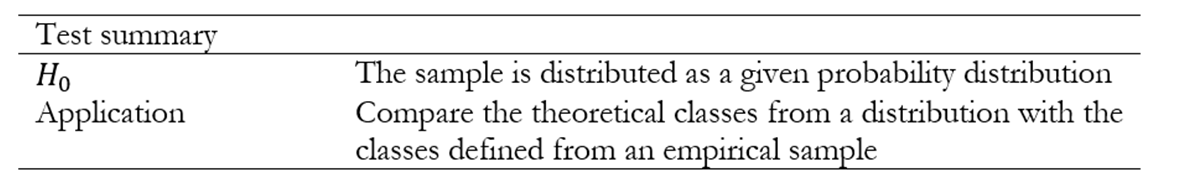
\includegraphics[width=0.9\textwidth]{SectionLetsMath/elemStat_figures/tab_Chi2.png}
\captionsetup{type=table}
\caption{$\chi^2$ test summary}
\label{tab_Chi2}
\end{figure}

\subsection{F-test}
This test aims at checking if two samples are normally distributed with the same variance. The statistics of this test is distributed as a Fisher-Snedecor distribution.
\begin{equation}
F=\frac{\frac{N_1}{m}}{\frac{N_2}{n}}
\label{eq_FisherDistribution}
\end{equation}

Where $N_1$ and $N_2$ are independent random variable $\chi^2$ distributed with $m$ and $n$ degrees of freedom. The test assumes $X$ and $Y$ are normally distributed. $X$ has $n$ samples and $Y$ has $m$ samples. The null hypothesis is $H_0=\sigma_X^2=\sigma_Y^2$. The statistic follows a Fisher distribution with $n-1$ and $m-1$ degrees of freedom:
\begin{equation}
F=\frac{S_X^2}{S_Y^2}
\label{eq_FisherTest1}
\end{equation}
The value of $F$ can be easily calculated having a dimensional space a number of $p$ parameters considering the sum of the squared residuals.
\begin{equation}
F=\frac{\left(\frac{SSR_X-SSR_Y}{p_X-p_Y}\right)}{\frac{SSR_Y}{n-p_Y}}
\label{eq_FisherTest2}
\end{equation}
The summary of the $F$-test is presented in Table \ref{tab_Ftest}.

% INSERT tab_Ftest
\begin{figure}[hbt!]
\centering
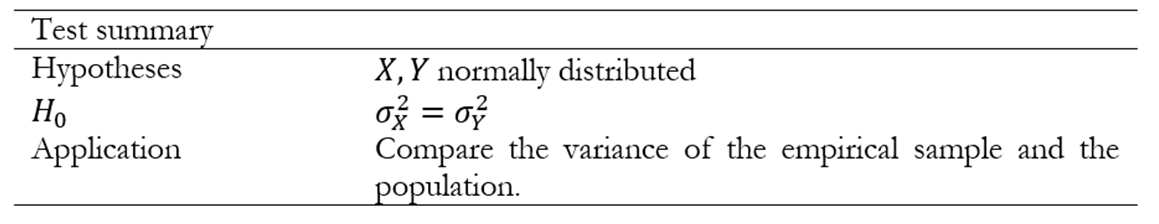
\includegraphics[width=0.9\textwidth]{SectionLetsMath/elemStat_figures/tab_Ftest.png}
\captionsetup{type=table}
\caption{F-test summary.}
\label{tab_Ftest}
\end{figure}

\section{Time series analysis} \label{secTimeSeries}


A time series (TS) is a series of the realisation of a random variable measured at constant time intervals. Time series can be used to forecast future values or to classify the realisations according to the properties of the TS (e.g., the seasonality). Even if both these applications sound intuitive, there is a lot of theory and math behind TSs. The entire theory of TS analysis is based on statistics.\par

The aim of TS analysis is the definition of a PDF describing the realisation of the events over time. Sometimes observations are some way linked to the others. This concept can be easily recognised thinking about the “continuity” of the nature around us (this is somehow related to the Principle of Least Action, already introduced in chapter \ref{sect_supplyChainPhysics}). Besides, it may exist a seasonality involving observations distant in the time (e.g. every summer is warmer than every winter). All these aspects drop the hypothesis of the independence of the observed variable that is commonly used in statistics to built simpler models. Under the independence hypothesis, it is possible to assume that the joint PDF of $X_1,\ldots,X_n$ random variables equals $f(x_1,\ldots,x_n)=\prod_{i=1}^{n}{f(x_i)}$. This is not true for TSs, and our work will get harder.\par

Since it is easy that each observation of a TS may depend on the previous: there is a sort of “influence” between them (in general, we can say that a TS has \textit{memory}). This is good news since it suggests that we could check historical values to make forecasts, that is one of our purposes.\par

TS are modelled as stochastic processes; for this reason, we introduce the notation indicating $X(\omega,t)$, where $X$ is the stochastic process. A TS behaves as a set of events $\omega$, one for each $t$ step, generated by $X(\omega,t)$. The random variable $X_t$ models the event at each time period $t$. Figure \ref{fig_stochProcess} shows the inputs and outputs of a stochastic process. We aim at describing the generating process $X(\omega,t)$ modelling the behaviour of the process to make forecasts.

% INSERT fig_stochProcess
\begin{figure}[hbt!]
\centering
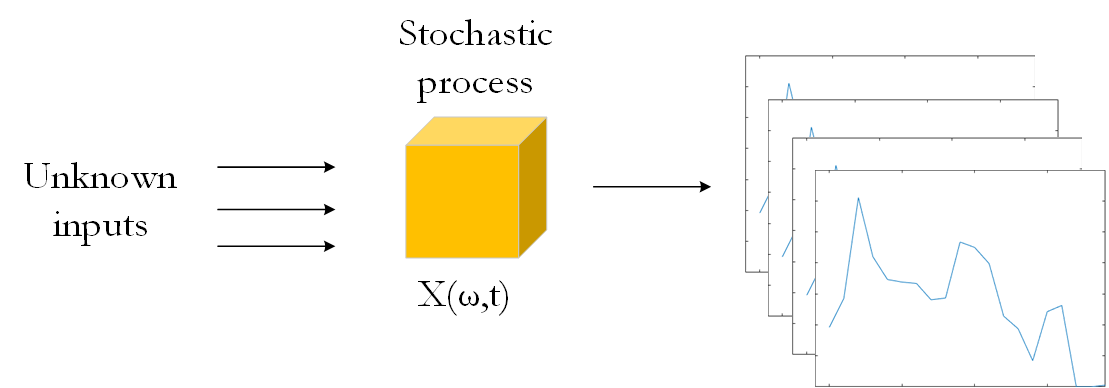
\includegraphics[width=0.9\textwidth]{SectionLetsMath/elemStat_figures/fig_stochProcess.png}
\captionsetup{type=figure}
\caption{Representation of a stochastic process.}
\label{fig_stochProcess}
\end{figure}


When modelling a TS as a stochastic process, there is a limit. A TS is composed of a single observation for each couple $(\omega,t)$. This is equal to have each event at a time $t$ represented by a single record (as having a single TS of the n represented in Figure \ref{fig_ACFPACF}). In practice, a single observation $X(t)$ is assumed to be representative of the entire event $\omega$ at time $t$. \footnote{The package logproj provides methods to deal with time series \href{https://github.com/aletuf93/logproj/blob/master/logproj/stat_time_series.py}{here}.
}

\subsection{Time series decomposition} \label{secTimeSeriesDecomposition}
TS decomposition is one of the approaches used to estimate the parameters of a stochastic process. The first assumption is made on how the stochastic process works. It is assumed it generates the TS based on three independent components.
\begin{itemize}
    \item A trend component $T(t)$;
    \item A seasonal component $S(t)$;
    \item A residual (random) component $R(t)$.
\end{itemize}

The literature proposes two models to mix these components. An additive (see equation \ref{eq_additiveTS}) and a multiplicative model (see equation \ref{eq_multiplicativeTS}). Figure \ref{fig_addMulTS} illustrates two realisations of an additive a multiplicative model.\footnote{The source code of Figure \ref{fig_addMulTS} is available \href{https://github.com/aletuf93/logproj/blob/master/examples/03.\%20Statistics.ipynb}{here}.}

\begin{equation}
X\left(t\right)=T\left(t\right)+S\left(t\right)+R(t)
\label{eq_additiveTS}
\end{equation}

\begin{equation}
X\left(t\right)=T\left(t\right)\times S\left(t\right)\times R(t)
\label{eq_multiplicativeTS}
\end{equation}

% INSERT fig_addMulTS
\begin{figure}[hbt!]
\centering
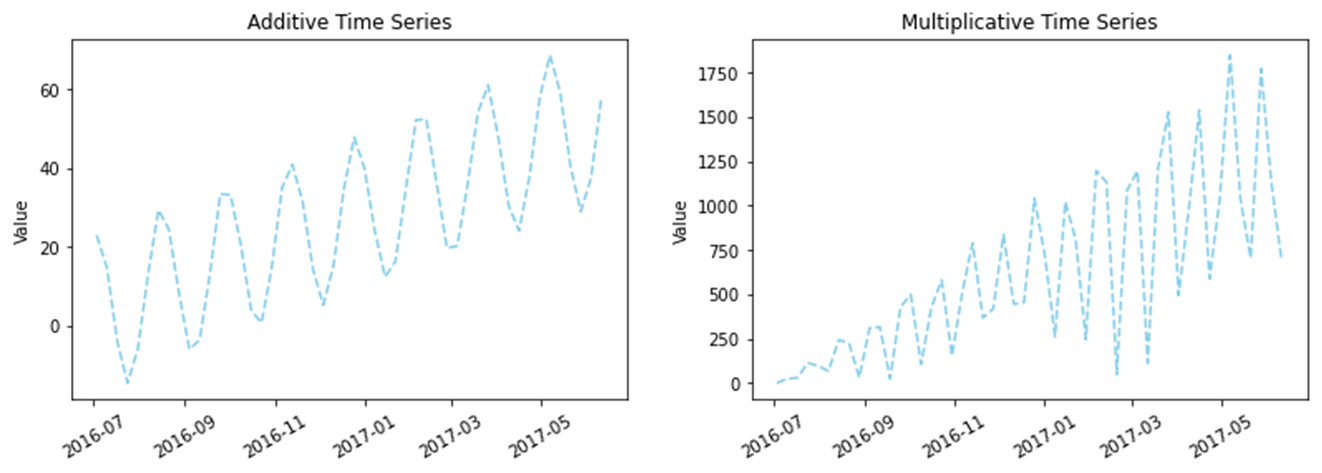
\includegraphics[width=0.9\textwidth]{SectionLetsMath/elemStat_figures/fig_addMulTS.png}
\captionsetup{type=figure}
\caption{Comparison between additive and multiplicative time series}
\label{fig_addMulTS}
\end{figure}

For the sake of brevity, the following paragraphs consider a TS modelled through additive model (see equation \ref{eq_additiveTS}) given that a multiplicative series can be transformed into an additive one using a logarithm transformation.

\begin{equation}
\begin{split}
    \log{\left(X\left(t\right)\right)} & =\log{\left(T\left(t\right)\times S\left(t\right)\times R\left(t\right)\right)}=\\
    & =\log{(T(t))+\log{(S(t))+\log{R(t))}}}\\
\end{split}
\label{eq_additiveMultiplicativeTransform}
\end{equation}

For this reason, all the techniques here presented are applicable to multiplicative models (see equation \ref{eq_multiplicativeTS}) too. In practice, one can fit both of them and measure their goodness of fit choosing the model which better describe the empirical measurements. 

An option to fit an additive model is to get the trend component of the series as a linear regression model fitted by ordinary least square (OLS\footnote{Section \ref{secLinearRegression} provides additional details of the OLS method.}). The result is a function $T\left(t\right)=mt+q$ where $m$ is the angular coefficient and $q$ is the intercept of the straight line best approximating the trend of $X(t)$. Alternatively, the trend can be estimated using a smoothing function, for example, using a Moving Average (MA) with a time window equal to the seasonality of $X(t)$\footnote{Sometimes, the seasonality of $X(t)$ is unknown. Section \ref{secFourier} shows how to detect the seasonality of a TS.}. Equation \ref{eq_trendTS} illustrates the formula of the MA; the time window is equal to $2h+1$ (e.g., $2h+1=7$ for a weekly seasonality of a time series having one sample per day).

\begin{equation}
T_t=\frac{1}{2h+1}\sum_{i=t-h}^{t+h}X_i
\label{eq_trendTS}
\end{equation}

Once the trend component T(t) has been extracted, the residual part (see Figure \ref{fig_extractedTrend})  of the TS equals\footnote{The source code of Figure \ref{fig_extractedTrend} is available \href{https://github.com/aletuf93/logproj/blob/master/examples/03.\%20Statistics.ipynb}{here}.}: 

\begin{equation}
S(t)+R(t)=X(t)-T(t)
\label{eq_extractedTrend}
\end{equation}

% INSERT fig_extractedTrend
\begin{figure}[hbt!]
\centering
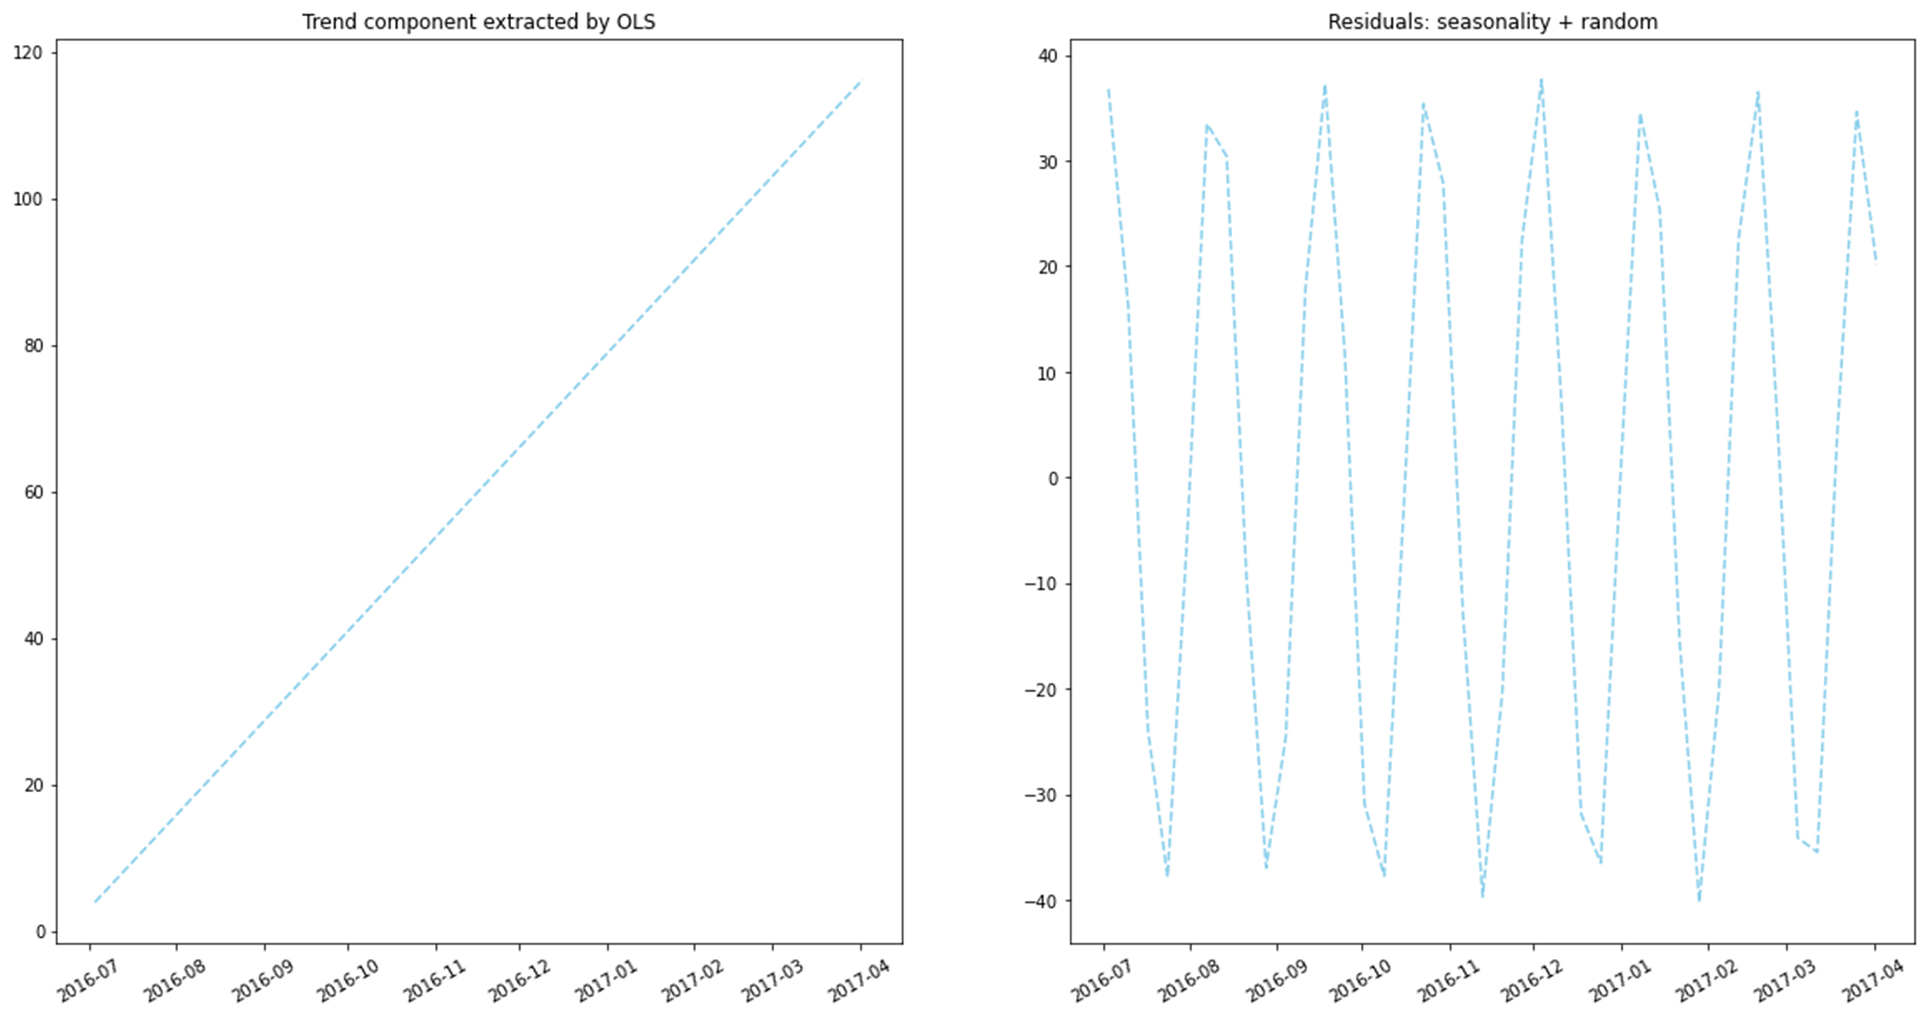
\includegraphics[width=0.9\textwidth]{SectionLetsMath/elemStat_figures/fig_extractedTrend.png}
\captionsetup{type=figure}
\caption{Extraction of the trend component from the TS.}
\label{fig_extractedTrend}
\end{figure}

To estimate the seasonal component $S(t)$ averaging is performed on the residual series $S\left(t\right)+R(t)$. Averaging works by grouping all the observation of the same seasonal period and applying average on it. The resulting value defines $S_t$. It is necessary to know the seasonality period to perform averaging (see Figure \ref{fig_averaging}). This can be done by the visualisation of the graphs or analytically using the Fourier transform analysing the frequency domain of the TS (see Section \ref{secFourier}).

% INSERT fig_averaging
\begin{figure}[hbt!]
\centering
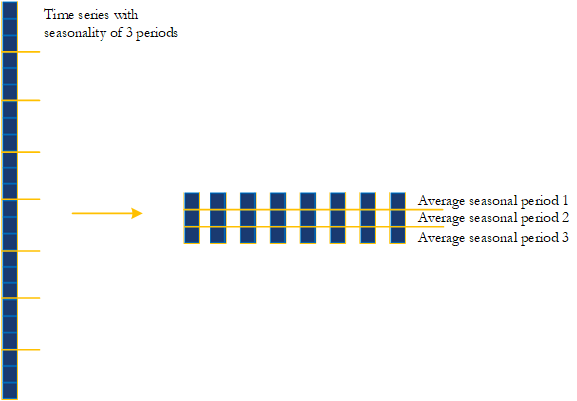
\includegraphics[width=0.9\textwidth]{SectionLetsMath/elemStat_figures/fig_averaging.png}
\captionsetup{type=figure}
\caption{Visualisation of the averaging method to estimate $S(t)$}
\label{fig_averaging}
\end{figure}

The residuals $R_t$ are obtained, again, by subtraction. If the residuals are randomly distributed, our model is interpreting the behaviour of the TS correctly. Otherwise, if the residuals show a pattern,  the estimation of $T(t)$ and $S(t)$ need more accuracy, or the choice of additive or multiplicative model is wrong. Figure \ref{fig_extractedSeasonality} shows the seasonal component and residuals. The residuals are randomly distributed, and it is possible to conclude that the decomposition process worked properly. Nevertheless, their magnitude is significant; collecting a higher number of samples would help in practice to reduce their magnitude and better detect the seasonality\footnote{The source code of Figure \ref{fig_extractedSeasonality} is available \href{https://github.com/aletuf93/logproj/blob/master/examples/03.\%20Statistics.ipynb}{here}.}.

% INSERT fig_extractedSeasonality
\begin{figure}[hbt!]
\centering
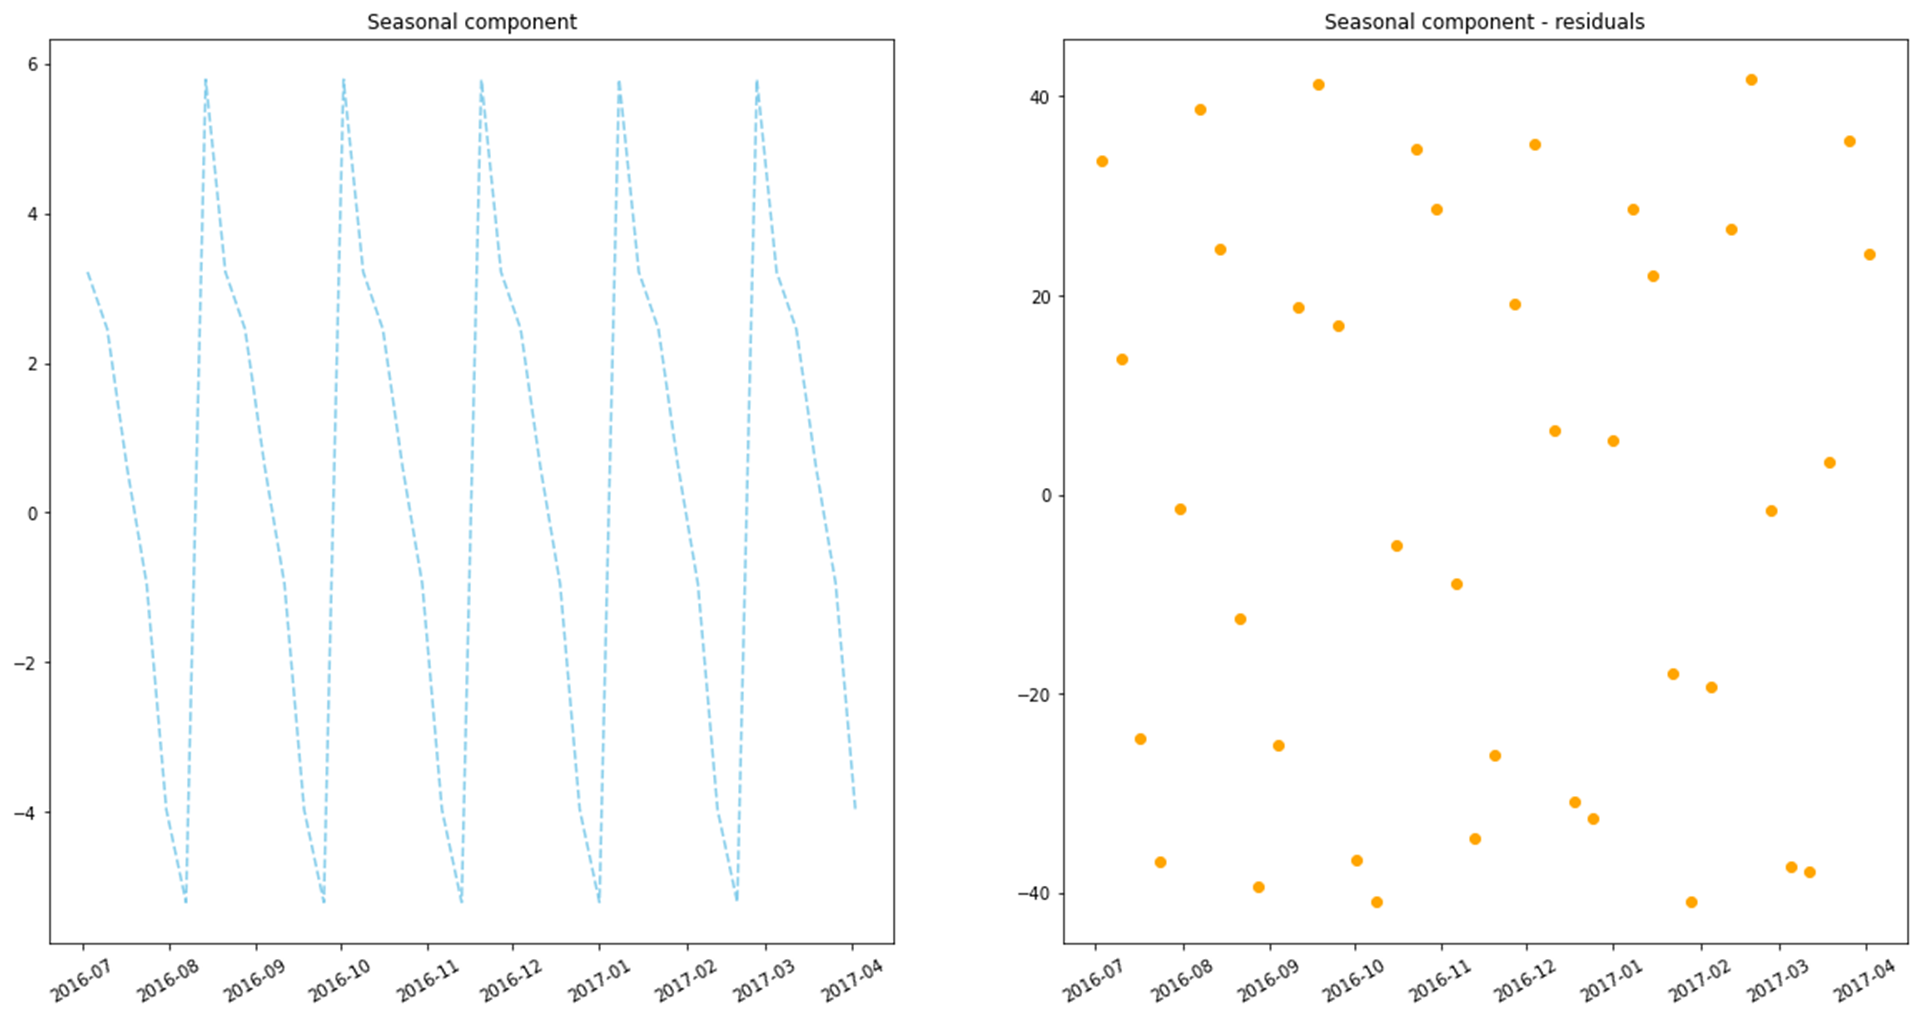
\includegraphics[width=0.9\textwidth]{SectionLetsMath/elemStat_figures/fig_extractedSeasonality.png}
\captionsetup{type=figure}
\caption{Extraction of the seasonal component from the TS.}
\label{fig_extractedSeasonality}
\end{figure}

\subsection{ARIMA models} \label{secARIMA}

A more complex way to model TSs comes from the autoregressive and moving average (ARIMA) models. These models are based on the Wold’s decomposition theorem stating that “Every covariance-stationary time series $X(t)$ can be written as the sum of two time series, one deterministic and one stochastic. In other words, given a stationary stochastic process $X_t$ with mean value $\mu$ it is always possible to decompose the process into $X_t=Z_t+V_t$ such that $cov\left(Z_t,X_t\right)=0$. In particular:

\begin{equation}
V_t=\mu+\sum_{j=1}^{+\infty}\left[\alpha_j\sin{\left(\omega_jt\right)}+\beta_j\left(\omega_jt\right)\right],0\le\omega_j\le\pi
\label{eq_ARIMAautoregressive}
\end{equation}

\begin{equation}
Z_t=\sum_{j=0}^{+\infty}{\psi_ja_{t-j}}
\label{eq_ARIMAmovingaverage}
\end{equation}

Equation \ref{eq_ARIMAautoregressive} models the autoregressive component where $V_t$ is the deterministic part of the model; $\omega_j$ is a fixed frequency and $\alpha_j$ and $\beta_j$ are uncorrelated white noise \footnote{A white noise process $a_t \sim WN\left(0,\sigma_a\right)$ is such that: $E\left(a_t\right)=0$; $Var\left(a_t\right)=\sigma_a^2$; $cov\left(a_t,a_{t-k}\right)=0 \forall t\in T,\ k\neq0$.} processes. $Z_t$ (see equation \ref{eq_ARIMAmovingaverage}) is the stochastic process and it is a moving average of infinity order where $a_t$ is the prediction error. In practice, a consequence of the Wold’s theorem is that once a TS has been transformed into a stationary TS it can be modelled as a linear function of a white noise process.A stochastic process is stationary when it has constant mean and variance and its autocovariance only depends on the time lag k (not by the time t). Using equations:

\begin{equation}
\begin{split}
    E\left(X_t\right)=\mu<\infty,\ & \forall t\in T\\
    Var\left(X_t\right)=\sigma_X^2<\infty,\ & \forall t\in T\\
    Cov\left(X_t,X_{t-k}\right)=\gamma_k<\infty,& \forall k\in T\\
\end{split}
\label{eq_stationarity}
\end{equation}

If these conditions are met, it is possible to apply an ARIMA model to a TS to model it as a sum of an autoregressive process (AR) (derived from $V_t$) and a moving average process (MA) (derived from $Z_t$). In general, a TS is not stationary, and it is not possible to directly apply ARIMA models. A trend in the series, for example, violates equations \ref{eq_stationarity}. For this reason, detrending is almost always necessary to get a series meeting the stationarity condition. Box and Jenkins \cite{Box1970} introduced some transformation to deal with non-stationary TS (see Table \ref{tab_transformation}).


% INSERT tab_transformation
\begin{figure}[hbt!]
\centering
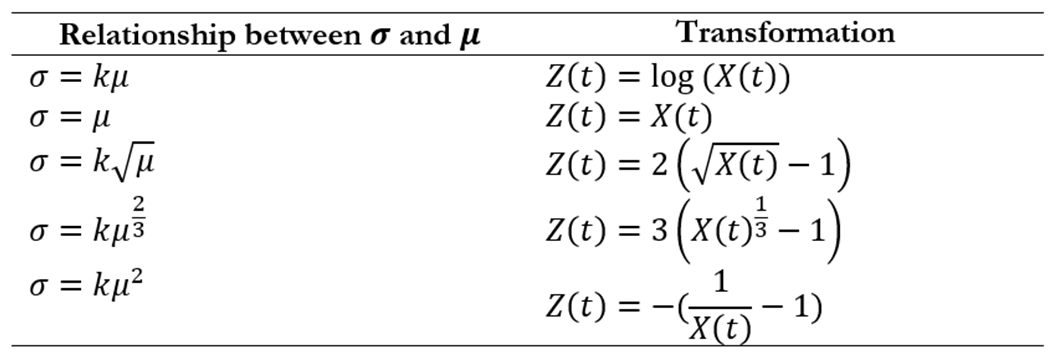
\includegraphics[width=0.9\textwidth]{SectionLetsMath/elemStat_figures/tab_transformation.png}
\captionsetup{type=table}
\caption{Transformations to obtain a stationary TS}
\label{tab_transformation}
\end{figure}


Once the TS has been transformed into a stationary one, it is possible to fit an ARIMA model choosing adequate parameters $p$ and $q$, indicating the autoregressive (AR) order and the moving average (MA) order. At this purpose, the autocorrelation functions PACF, and ACF are studied. The echo phenomenon exemplifies the effect of the autocorrelation. After a certain amount of time units (i.e. time lags), the echo overlaps original message altering the sound waveform. The echo of the signal of a TS is the seasonality (i.e. certain weeks or months of the year where the TS is amplified). To detect this phenomenon, we use ACF and PACF as defined in Section \ref{secCovarianceCorrelation}. Figure \ref{fig_nonStationaryTS} illustrates a TS with its ACF and PACF, while Figure \ref{fig_StationaryTS} illustrates the same series with ACF and PACF after detrend using OLS.\footnote{The source code of Figure \ref{fig_nonStationaryTS}, and Figure \ref{fig_StationaryTS} is available \href{https://github.com/aletuf93/logproj/blob/master/examples/03.\%20Statistics.ipynb}{here}.}.


% INSERT fig_nonStationaryTS
\begin{figure}[hbt!]
\centering
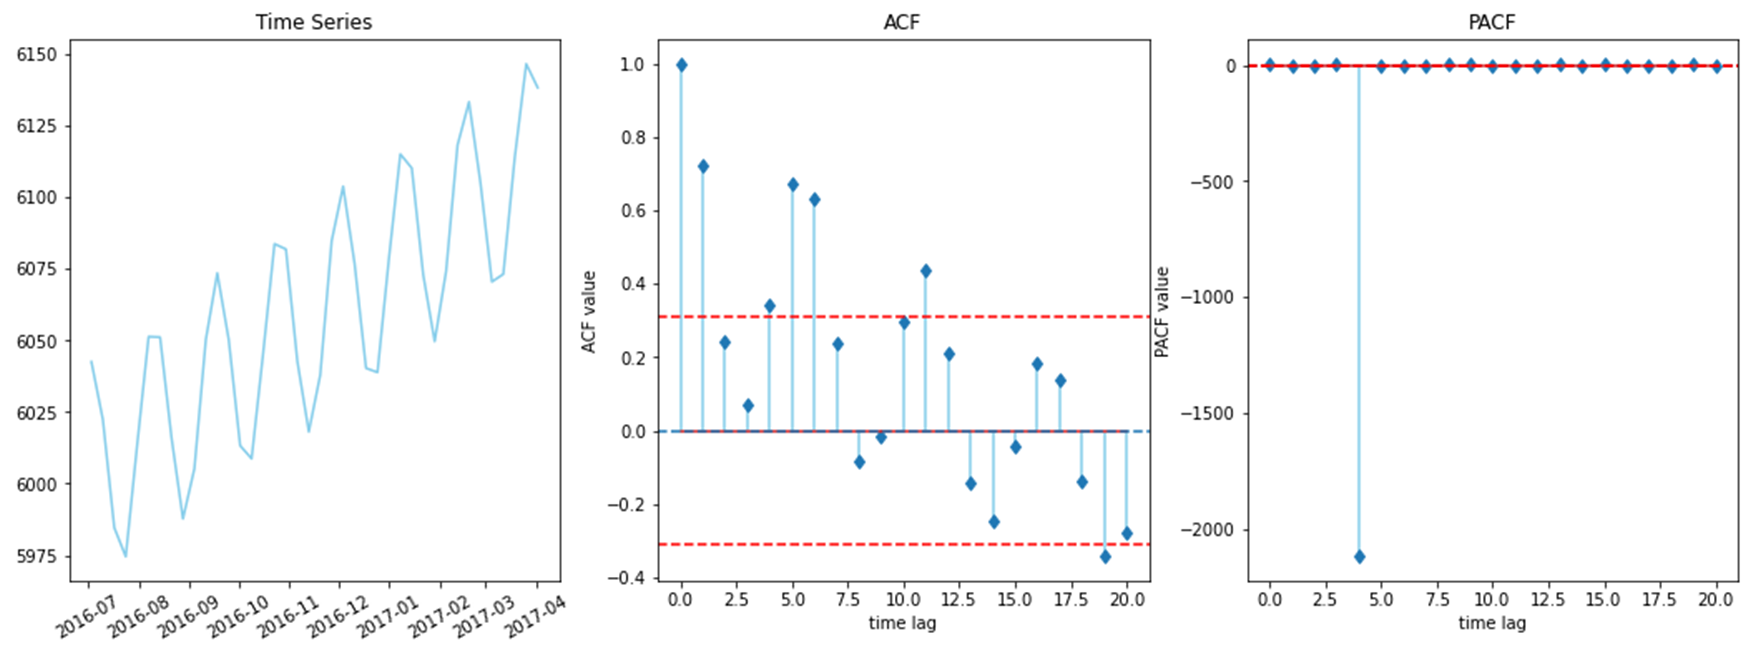
\includegraphics[width=0.9\textwidth]{SectionLetsMath/elemStat_figures/fig_nonStationaryTS.png}
\captionsetup{type=figure}
\caption{ACF and PACF of the original TS.}
\label{fig_nonStationaryTS}
\end{figure}

% INSERT fig_StationaryTS
\begin{figure}[hbt!]
\centering
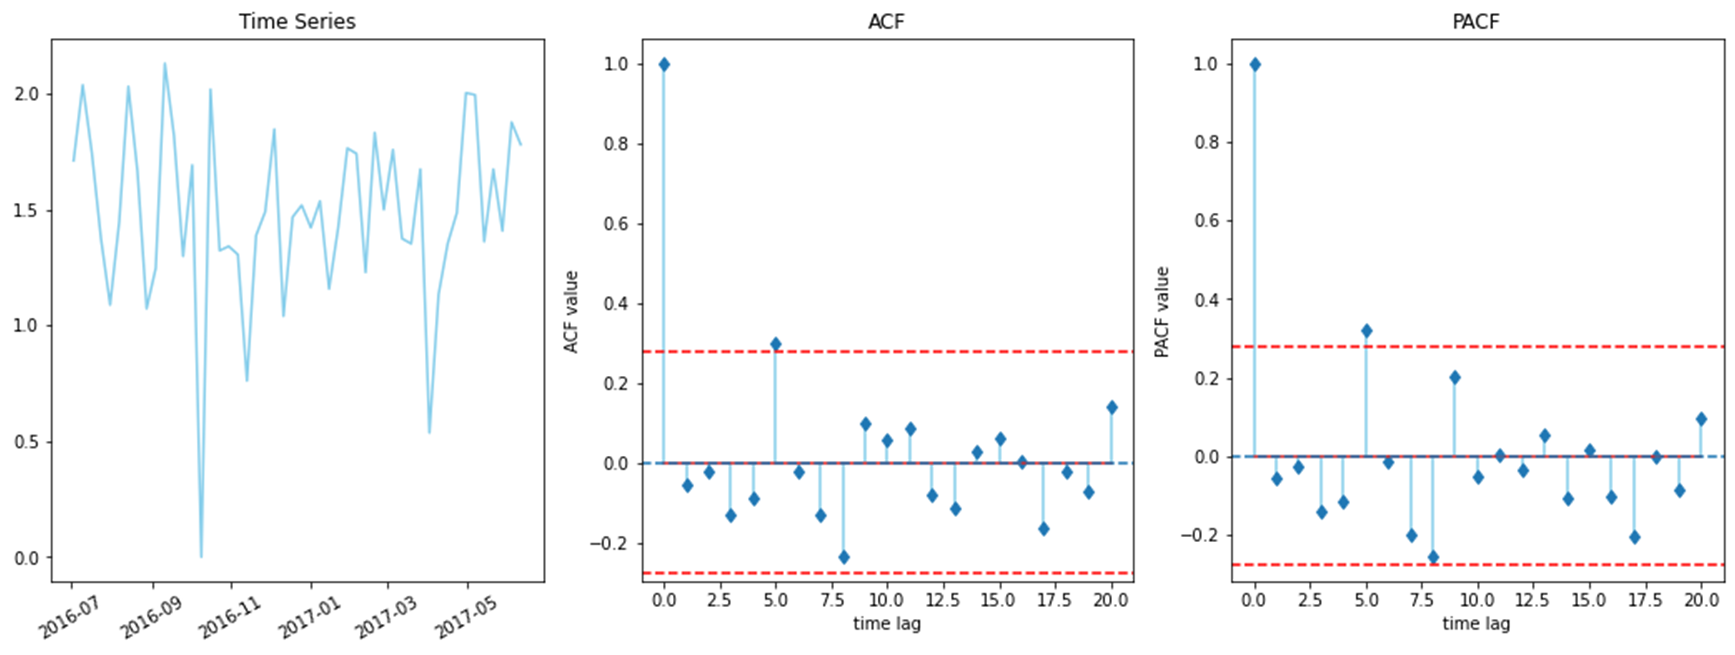
\includegraphics[width=0.9\textwidth]{SectionLetsMath/elemStat_figures/fig_StationaryTS.png}
\captionsetup{type=figure}
\caption{ACF and PACF of the detrended TS.}
\label{fig_StationaryTS}
\end{figure}

Stationarity can be tested using the Dickey-Fuller test for stationarity. Alternatively, a series is stationary if its ACF and PACF decrease, i.e. the ACF, and PACF correlograms tends to zero asymptotically. The last significant value of the PACF is used for the parameter $p$ (the order of the AR model) while the last significant lag value of the ACF is used for the parameter $q$ (the order of the MA model). In this case, we would try to fit a model ARIMA(1,1). Note that if the PACF goes to zero immediately, the most important value is '1' (since a TS is always autocorrelated with itself at the same time lag). In this case, $T_t$ is constant and no waveform (i.e. seasonality) exists. When the ACF suggests no values, instead, '0' should be the order used for $q$.

\subsection{Fourier transform} \label{secFourier}

All the models introduced in the previous paragraphs assume that a seasonality exists and its lag is defined (or can be defined analysing the graph of the time series). Nevertheless, in some cases, it may be necessary to have analytical methods to study the seasonality of a series. For this reason, we introduce the spectrum analysis and the Fourier transform. Spectrum analysis is a methodology widely used in telecommunication for the analysis of signals. Signals (analogue or digital) are usually periodic and characterised by a period $\tau$, due to their sinusoidal behaviour. A periodic (i.e. sinusoidal) signal (see Figure \ref{fig_signal}) can be modelled as\footnote{The source code of Figure \ref{fig_signal} is available \href{https://github.com/aletuf93/logproj/blob/master/examples/03.\%20Statistics.ipynb}{here}.}.:

\begin{equation}
y=S(t)=Asin(\omega t+\phi)
\label{eq_signal}
\end{equation}


% INSERT fig_signal
\begin{figure}[hbt!]
\centering
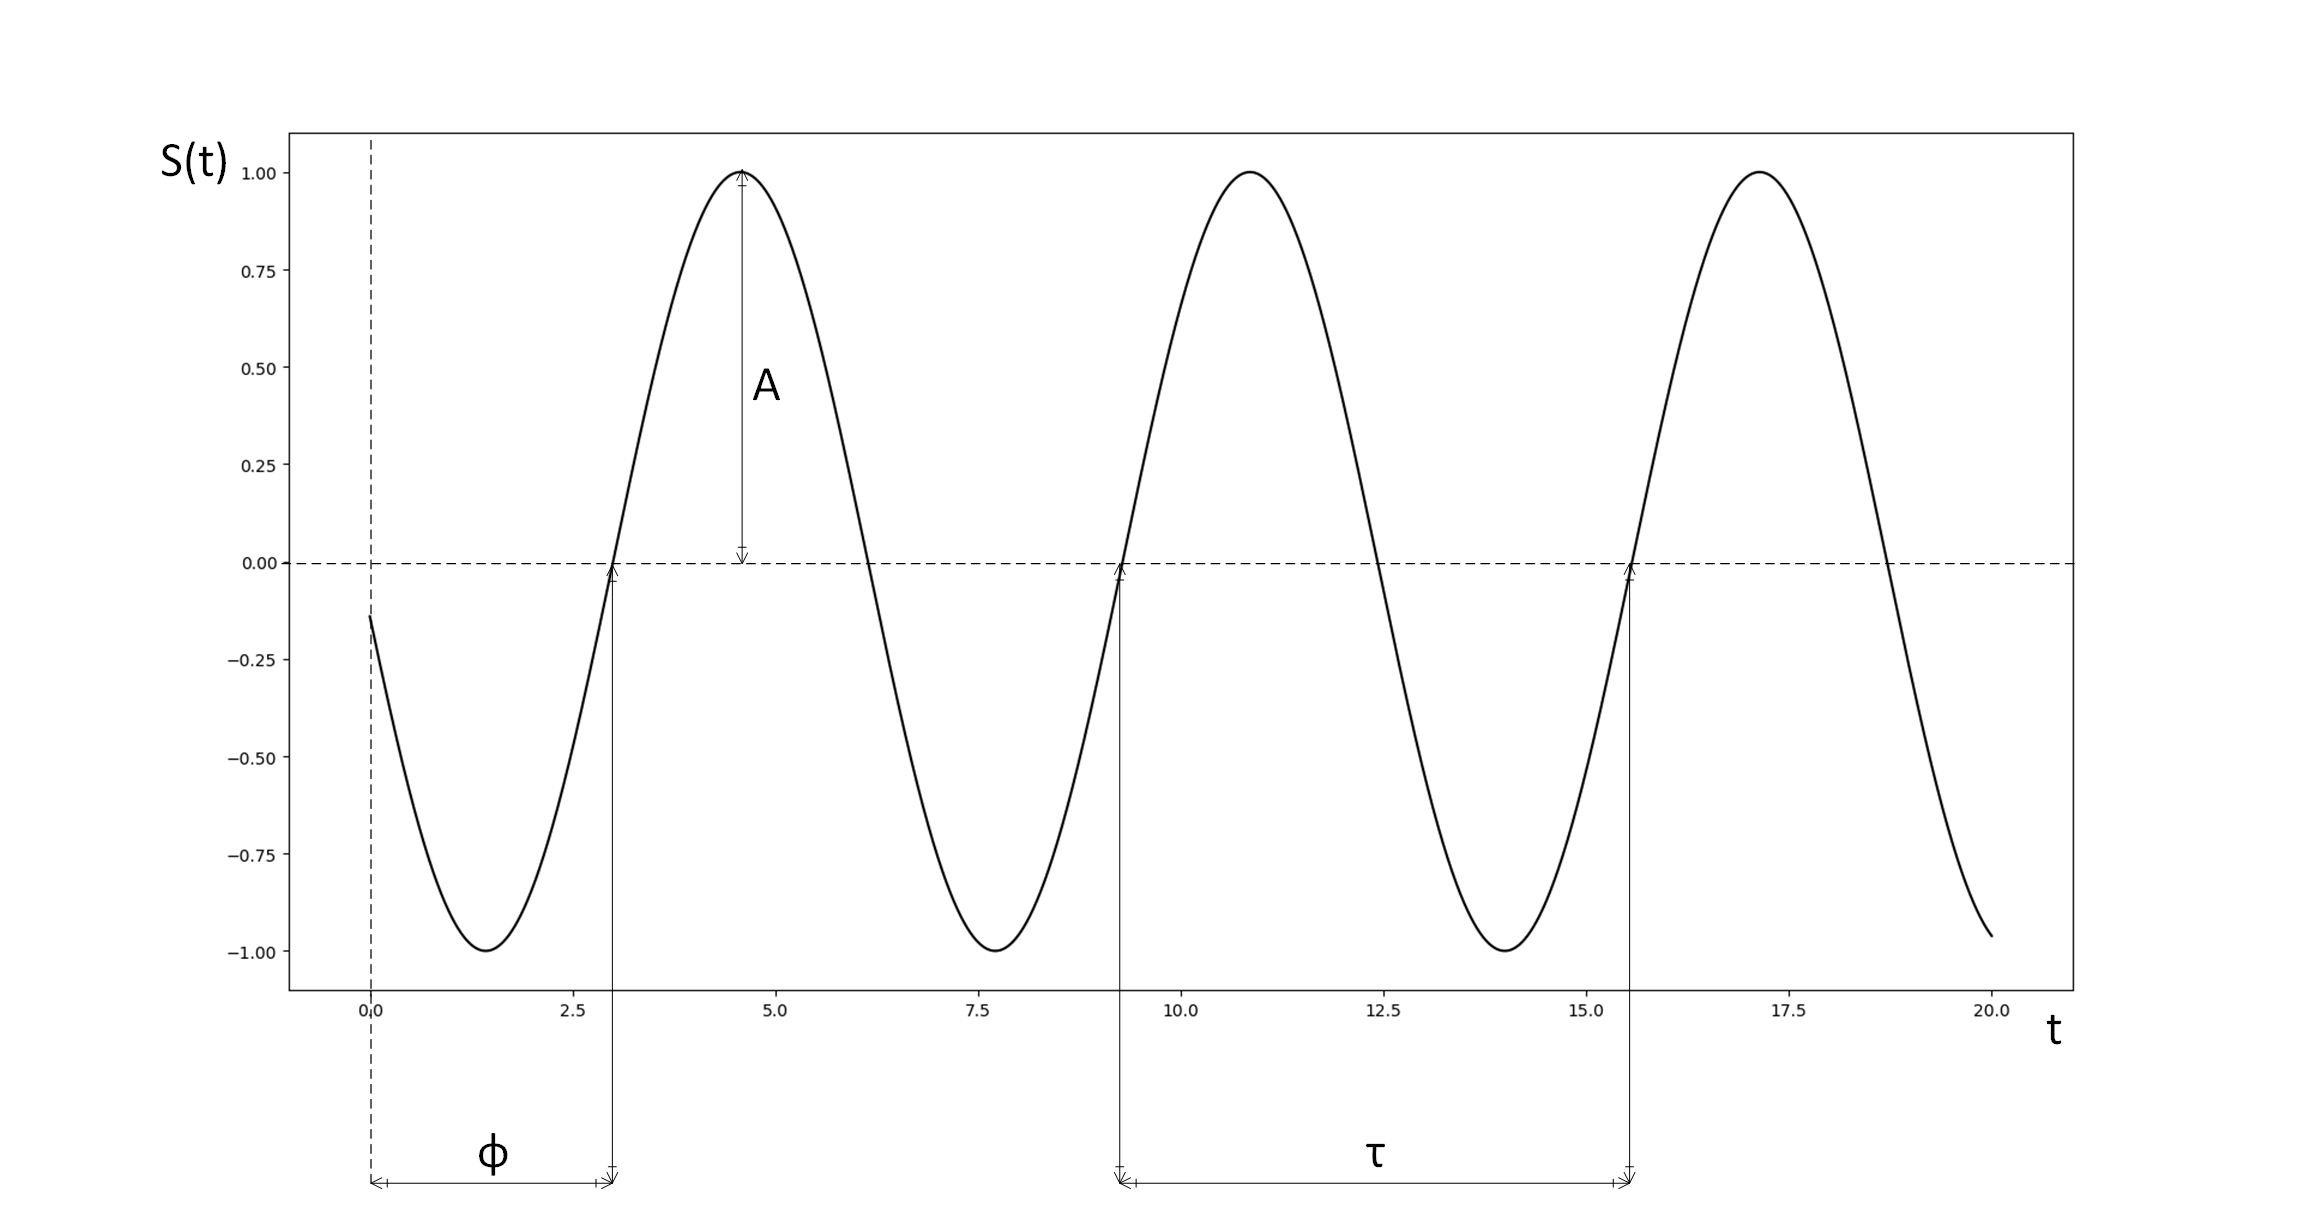
\includegraphics[width=0.9\textwidth]{SectionLetsMath/elemStat_figures/fig_signal.png}
\captionsetup{type=figure}
\caption{Model of a periodic signal.}
\label{fig_signal}
\end{figure}

Where $A$ is the amplitude of the signal, $\phi$ is the phase (translation on the time axis). $\omega$ is the angular velocity, i.e. the number of periods within a time interval of $2\pi$. The frequency $f$ is linked to the period $\tau$ and to the angular velocity $\omega$ by the following.

\begin{equation}
f=\frac{1}{\tau}=\frac{\omega}{2\pi}
\label{eq_frequency}
\end{equation}

Given the equation \ref{eq_frequency}, the $S\left(t\right)$ can be expressed in terms of the frequency $f$.

\begin{equation}
y=Asin(f2\pi t+\phi)
\label{eq_frequency2}
\end{equation}

Telecommunication uses different strategies to transmit signals avoiding losses during the transmission. It often happens to transmit signals digitally. When the source is analogue (i.e. continuous bu nature) the signal has to be sampled. Sampling means removing part of the signal, but if it is performed correctly, it does not remove any information. Sampling is performed at a fixed frequency $f_s$ i.e., each sample has a distance in time from the previous one equal to $T$. To properly maintain the level of information of a signal, $f_s$ must be chosen adequately. The Nyquist-Shannon sampling theorem demonstrates that given a periodic signal $g\left(t\right)$ with maximum frequency $f_M$ (i.e. a bandwidth $[0,f_M]$), can be completely defined (i.e. without loss of information) using a sampling frequency $f_s\geq2f_M$ i.e. a sampling step $t_s\le\frac{1}{2f_M}$. Figure \ref{fig_signalsampling} shows the samples of a signal generated by a continuous source.\footnote{The source code of Figure \ref{fig_signalsampling} is available \href{https://github.com/aletuf93/logproj/blob/master/examples/03.\%20Statistics.ipynb}{here}.}


% INSERT fig_signalsampling
\begin{figure}[hbt!]
\centering
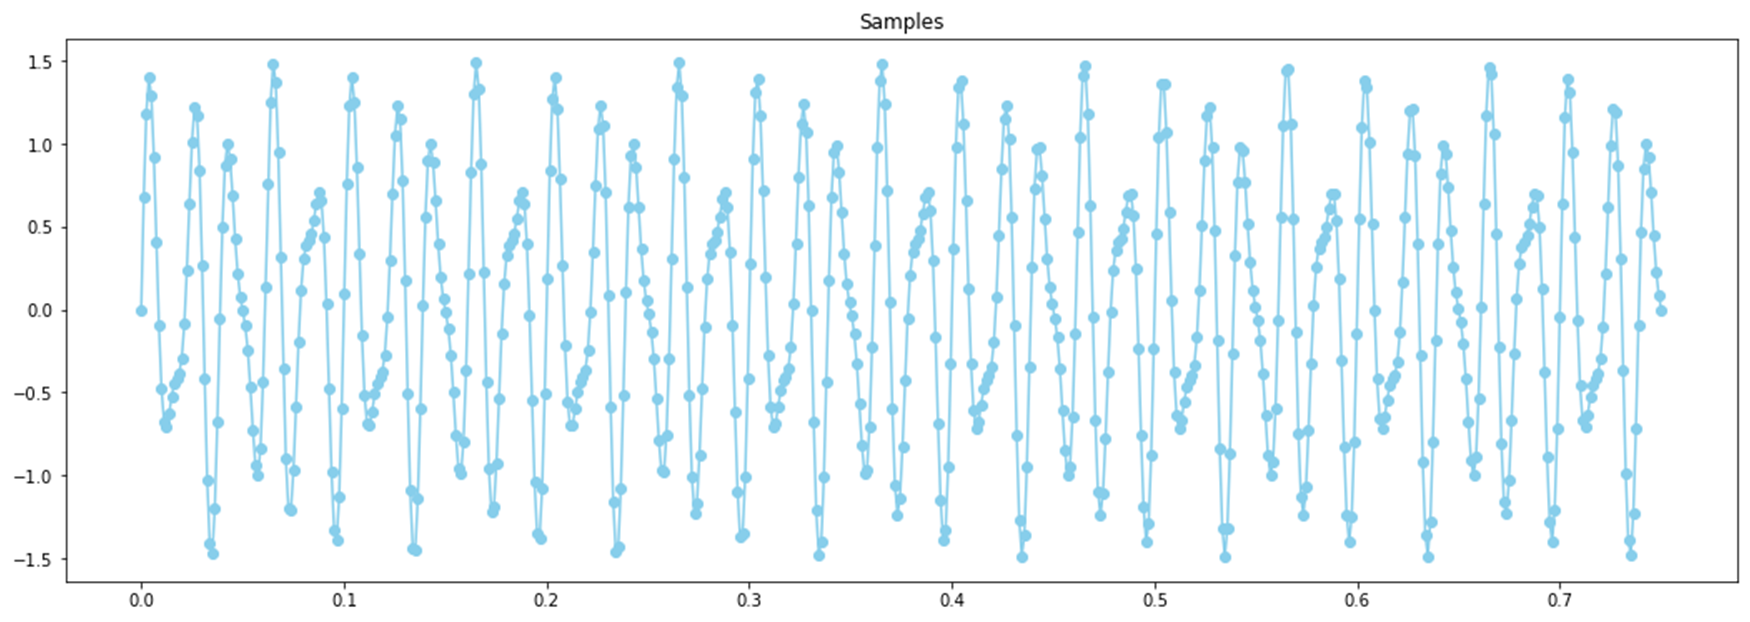
\includegraphics[width=0.9\textwidth]{SectionLetsMath/elemStat_figures/fig_signalsampling.png}
\captionsetup{type=figure}
\caption{signal with $N=600$ and $f_s\ =800\ $ Hz.}
\label{fig_signalsampling}
\end{figure}

The original signal can be recreated using the Fourier transform on the sampled signal investigating its behaviour in the frequency domain. The signal is expected to have a maximum original frequency of 400\ Hz (i.e. it has been sampled correctly, accordingly with the Nyquist-Shannon theorem).\par

The Fourier theorem states that any periodic function $x(t)$ may be expressed as a sum of infinite terms of sine and cosine terms (called Fourier series), each of them with a specific amplitude and phase complex coefficient $c_n$ called the Fourier coefficient. 

\begin{equation}
c_n=\frac{1}{T_0}\int_{T_0}{x\left(t\right)e^{-2\pi n f_0t\ }dt}
\label{eq_FourierCoefficients}
\end{equation}

Fourier transform is used to calculate the values of $c_{n\ }$.

\begin{equation}
X\left(f\right)=F\left\{x\left(t\right)\right\}=\int_{-\infty}^{+\infty}{x\left(t\right)e^{-j2\pi ft}}dt
\label{eq_Fouriertransform}
\end{equation}

The representation of these frequencies is obtained through amplitude and phase spectra which represents the absolute value and the argument of the complex coefficients $c_n$. The amplitude spectrum of the sampled signal is shown in Figure \ref{fig_Fourier}.\footnote{The source code of Figure \ref{fig_Fourier} is available \href{https://github.com/aletuf93/logproj/blob/master/examples/03.\%20Statistics.ipynb}{here}.}

% INSERT fig_Fourier
\begin{figure}[hbt!]
\centering
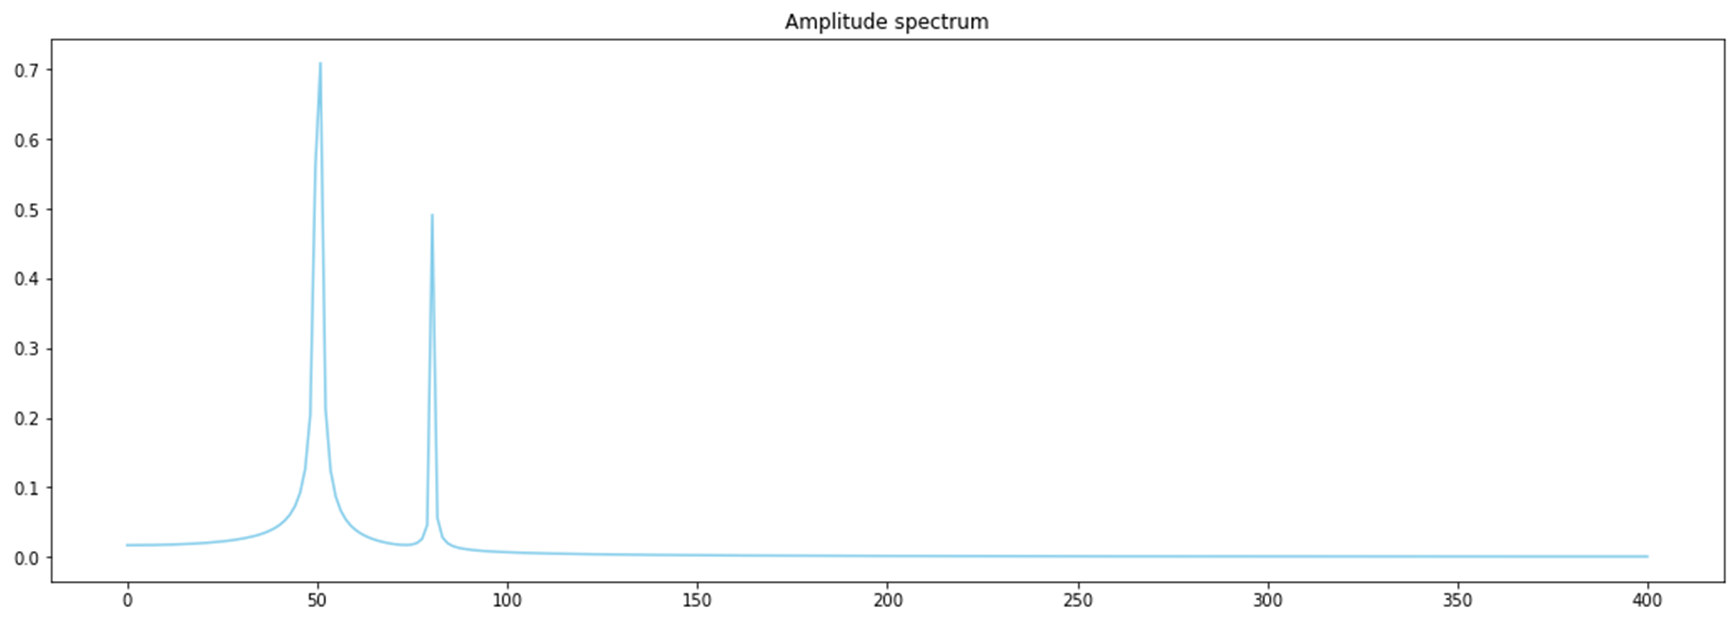
\includegraphics[width=0.9\textwidth]{SectionLetsMath/elemStat_figures/fig_Fourier.png}
\captionsetup{type=figure}
\caption{Amplitude spectrum of the signal.}
\label{fig_Fourier}
\end{figure}

The amplitude spectrum shows that two sinusoids with frequency 50 and 80 Hz generate the original signal; the harmonics are showed on the chart. Looking at the source code, the generating function of the samples was $y=\sin{\left(50 \times 2\pi x\right)}+0.5\sin(80\times2\pi x)$ which confirms the results of the transform.\par

Dealing with time series, we can use the Fourier transform to investigate if a periodical signal can be used to model the seasonal component of the series. In particular, we are looking for $f$ of the model in equation \ref{eq_frequency}. Where $f$ can be reasonably be expressed in $week^{-1}$, i.e. $f^{-1}$ defines the length of a period, i.e. the length of the seasonality.\par

Time series are usually extracted from a database which is digitalised and already sampled (e.g. daily/monthly/yearly) so it is difficult to define a priori the number of samples. This can be defined by different grouping strategy (e.g., daily/weekly). It is, anyway, essential to verify if the number of samples allows for resilient inference on the seasonality.\par

To perform Fourier analysis on a time series, it is necessary to detrend it first, as shown in \ref{secTimeSeriesDecomposition}. At this stage, the time series fluctuates around its mean with an unknown frequency and can be modelled as a periodic signal using the Fourier transform. 

\section{Bayesian Statistics} \label{secBayesTheorem}
The statistics illustrated so far is entirely based on the observation of physical phenomena. The events are observed, measured, and the outcomes of these experiments are analysed in a \textit{frequency} fancy. The values occurring the most are the most probable. This statistics is based on the frequentist approach. Sometimes we do not have the possibility of measure the variable of our interest; nevertheless, we have \textit{beliefs} on the behaviour of this variable, and we may be interested in expressing these believes in terms of probability. \par

For example, when measuring partial data of a total quantity, we have the belief that the total quantity is higher than the measured one. We can measure a variable using two different measurement systems, having the belief that one outperforms the other under certain circumstances. We may start an experiment having prior beliefs on the expected outcome. Bayesian statistics helps in all these situations. The main theorem of Bayesian statistic is the Bayes’ theorem:

\begin{equation}
P\left(A\middle| B\right)=\frac{P(A\cap B)}{P(B)}=\frac{P(B|A)}{P(B)}
\label{eq_bayesTheorem}
\end{equation}

This theorem is also known as the theorem of conditional probability. While frequentist statistics assume $A$, and $B$ being events; the Bayesian approach defines $A$ as the prior, and $B$ the posterior. The prior $A$ defines the belief we have before an experiment starts, i.e. before starting collecting measurement. The information of the measurements is, then, contained in the posterior $B$. Bayesian statistics aims at matching the prior and the posterior by assuming that the prior $A$ is true. In practice, we have observations, we expect they behave as $A$ describes, but we observe a behaviour $B$, and we need to correct it. Bayesian statistics is the perfect tool to match prior models with posterior empirical observations to predict their behaviour. Bayesian tools work similarly to machine learning models since all machine learning models aim at the definition of a joint probability distribution between a prior and a posterior. For this reason, these methods are presented in \ref{secBayesianMethods}.



\section*{Further reading}
Supplementary reading materials can be found in \cite{Sauter2002}, \cite{Ruppert2015}, \cite{Brandt2014}, \cite{Heibergerer2015}.

%\clearpage
\bibliographystyle{ieeetr}
\bibliography{SectionLetsMath/elemStat_ref}


